\documentclass{article}
\usepackage{amsmath}
\usepackage{graphicx}
\usepackage{placeins}
\usepackage[a4paper, portrait, margin=3cm]{geometry}
\begin{document}
\title{Human Capital in East and West Germany post reunification}
\author{Christian Koopmann}
\maketitle

\section{Introduction}
This study will analyse how the returns to experience and education evolved in East and West Germany in the years since reunification. The goal is to see to what extend differences in wage levels and the wage distribution can be attributed towards different evaluations of experience as well as education gathered before and after reunification. In the case of experience one hypothesis to test is that differences in returns to experience are mainly due to the low value of work experience from the GDR in the post reunification labour market. This study will follow a Human Capital based approach. Therefore this study will also attempt to estimate the Human Capital stored in the different types of education and experience by evaluating the returns to experience and education at the time specific mean levels. Since this also accounts for the different amounts of education and experience held in the respective sub-samples, it might give a clearer picture of the factors determining the wage structure. In order to determine how differences in human capital might vary for different demographic groups this analysis will also be done separately for different age and skill groups.

\section{Data and Descriptive Evidence}
The data used in this analysis consists of the data on all full time employed individuals in the A and C samples of the Socio Economic Panel. To slow the ageing and attrition of the sample individuals from later samples were also included when the amount of Old and New Experience or Education could still be inferred with reasonable accuracy. These include mainly younger individuals for whom education was finished after reunification and therefore all experience can be assumed to be New Experience. In this section several graphs are presented illustrating the development of mean wages as well as levels of education and experience across time and region. This is also done separating the data across the same dimensions (age and skill group) as in the later sections.
\subsection{Distribution of Wages}
In the following section several graphs describing the development of mean gross wages (deflated to 2010 prices) across time are presented.

Looking at the figures below one might draw the following conclusions about the wage distribution:

\begin{enumerate}
	\item Overall wages in East Germany rose quickly in the years after reunification. However wage growth then slowed down to a similar rate as in West Germany. At the end of the time frame significant differences persist (see Figure \ref{fig:MeanWages}).
	\item The wage distribution across overall experience started out very flat in East Germany but changed to resemble the structure in West Germany, although at lower total wage levels (see Figure \ref{fig:MeanWagesByTotalExp}). This seems to suggest returns to Total Experience in the East rising towards West German Levels over time.
	\item Wages in East Germany do not significantly differ with regards to Old Experience anywhere in the time frame (see Figure \ref{fig:MeanWagesByOldExp}). This suggest near zero returns to Old Experience in the East
	\item Wages in West Germany differ significantly across Old Experience immediately after Reunification, although those differences disappear over time (see Figure \ref{fig:MeanWagesByOldExp}). This suggests returns to Old Experience converging towards zero.
	\item The Wage Distribution across New Experience seems to be relative constant over time with no significant differences between East and West immediately visible, except for total levels (see Figure \ref{fig:MeanWagesByNewExp}). 
	\item There seem to be rising returns to education at the upper end of the education distribution (above 15 years) in East Germany (Figure \ref{fig:MeanWagesByTotalEdu}. This suggests rising returns to University Degrees which is confirmed by the analysis in Figure \ref{fig:MeanWagesBySkillGroup}
	\item There seems to be an overall rising wage inequality across age (see Figure \ref{fig:MeanWagesByAgeGroup}) which might be the result of the behaviour across experience described above.
\end{enumerate} 
 
\begin{figure}[!h]
    \centering
    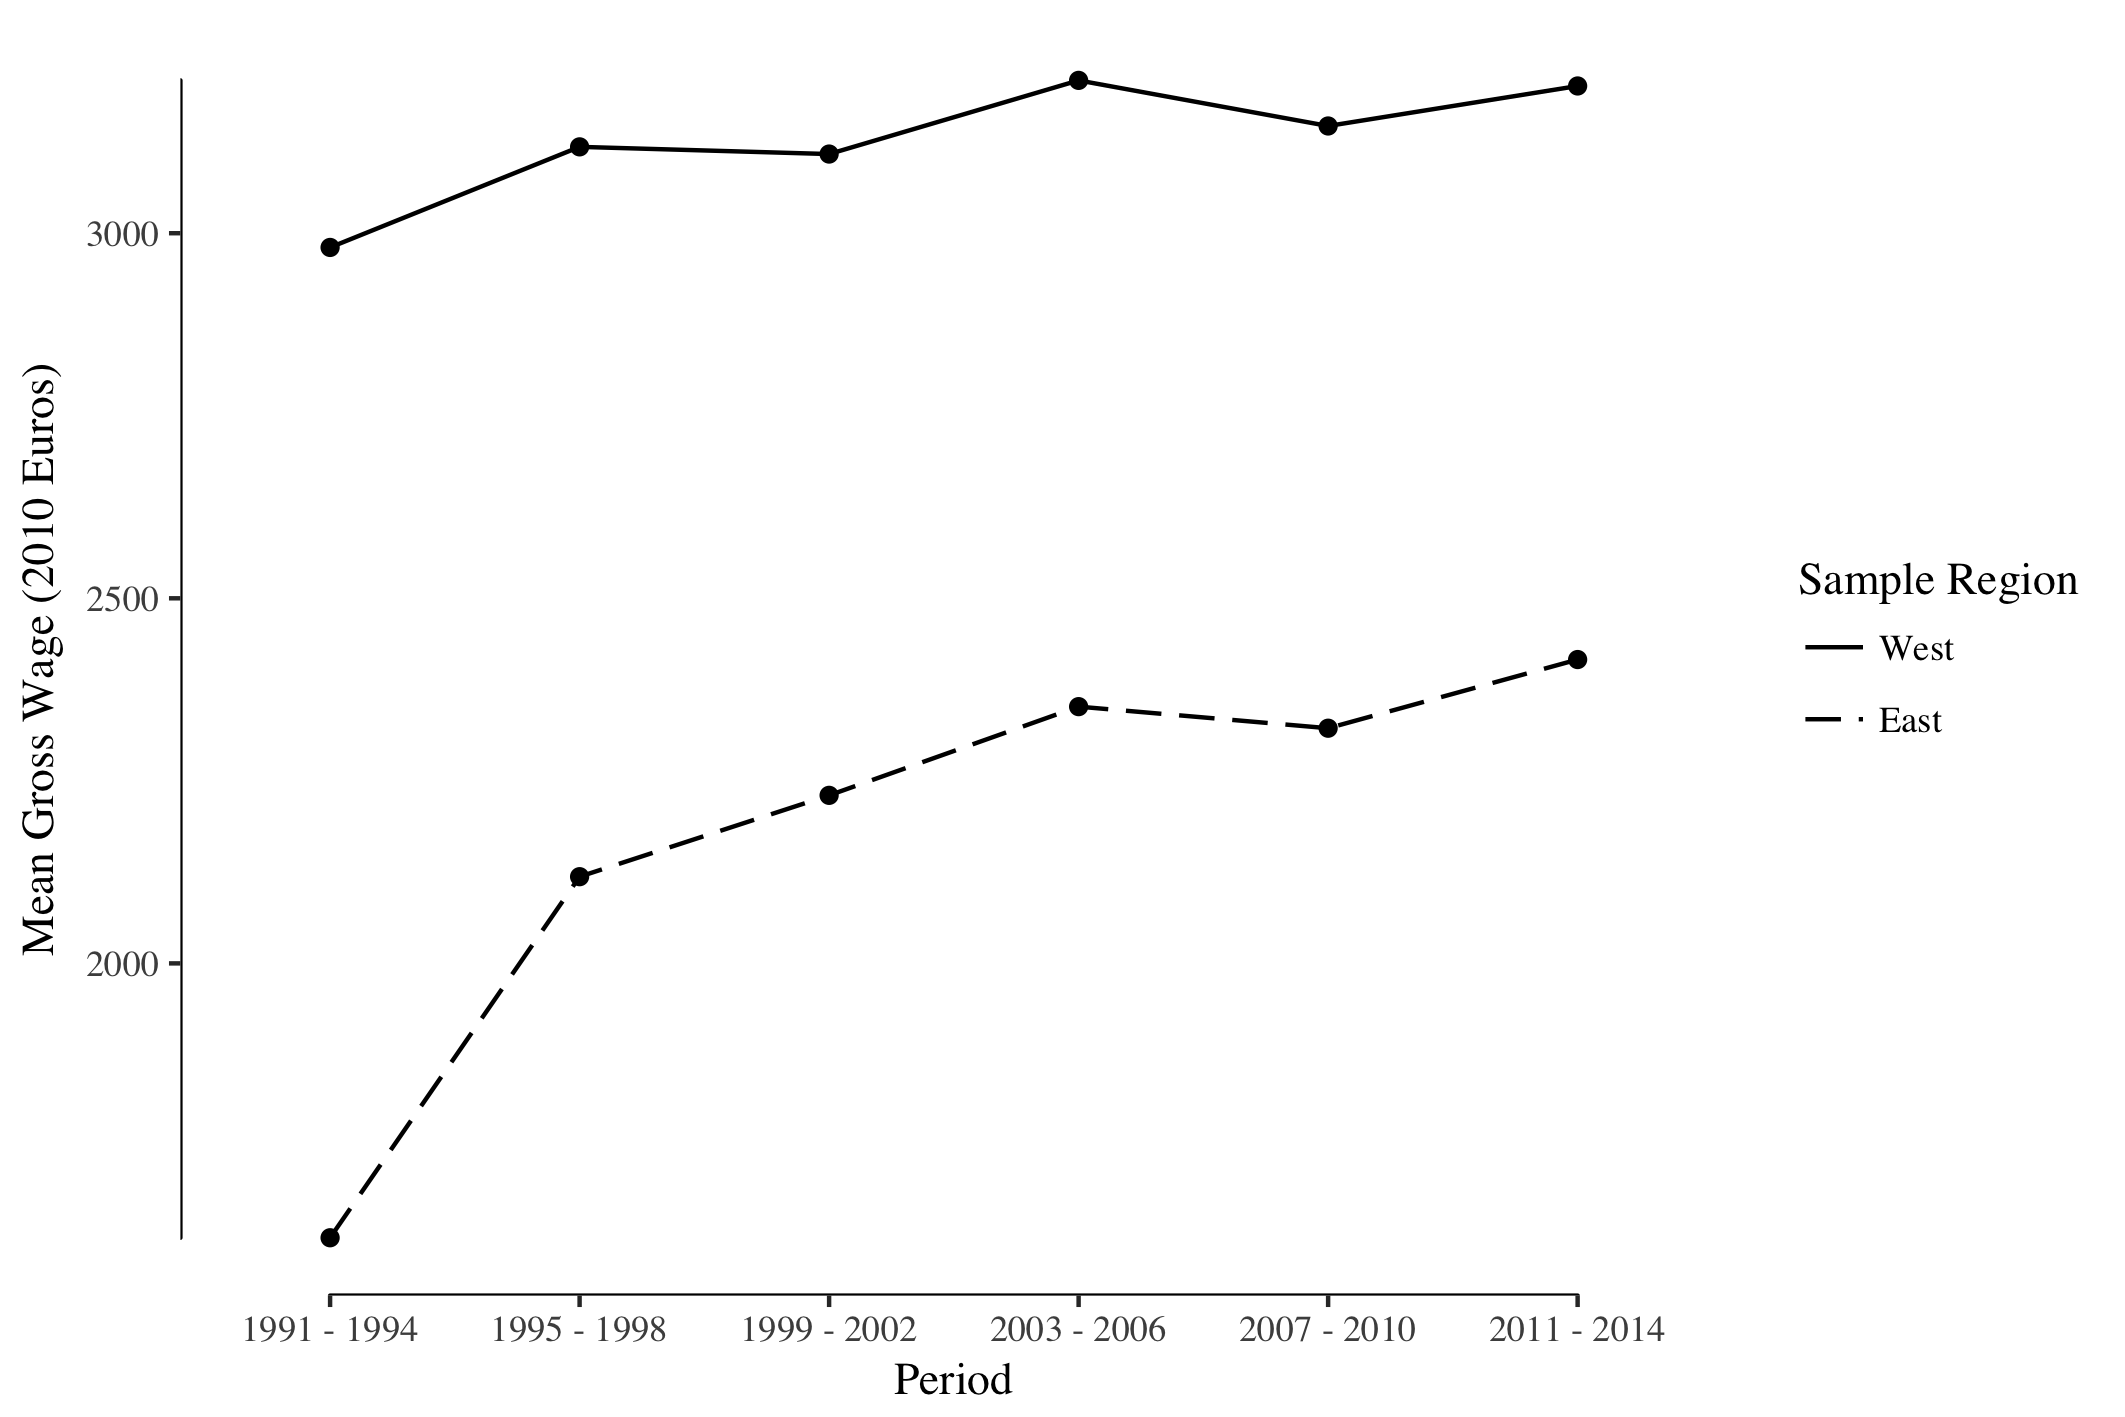
\includegraphics[width=\textwidth]{/Users/Christian/Statistik_Studium/EconProject/Code/Graphics/plotMeanWages.png}
    \caption{Average Wages}
    \label{fig:MeanWages}
\end{figure}

\begin{figure}[!h]
    \centering
    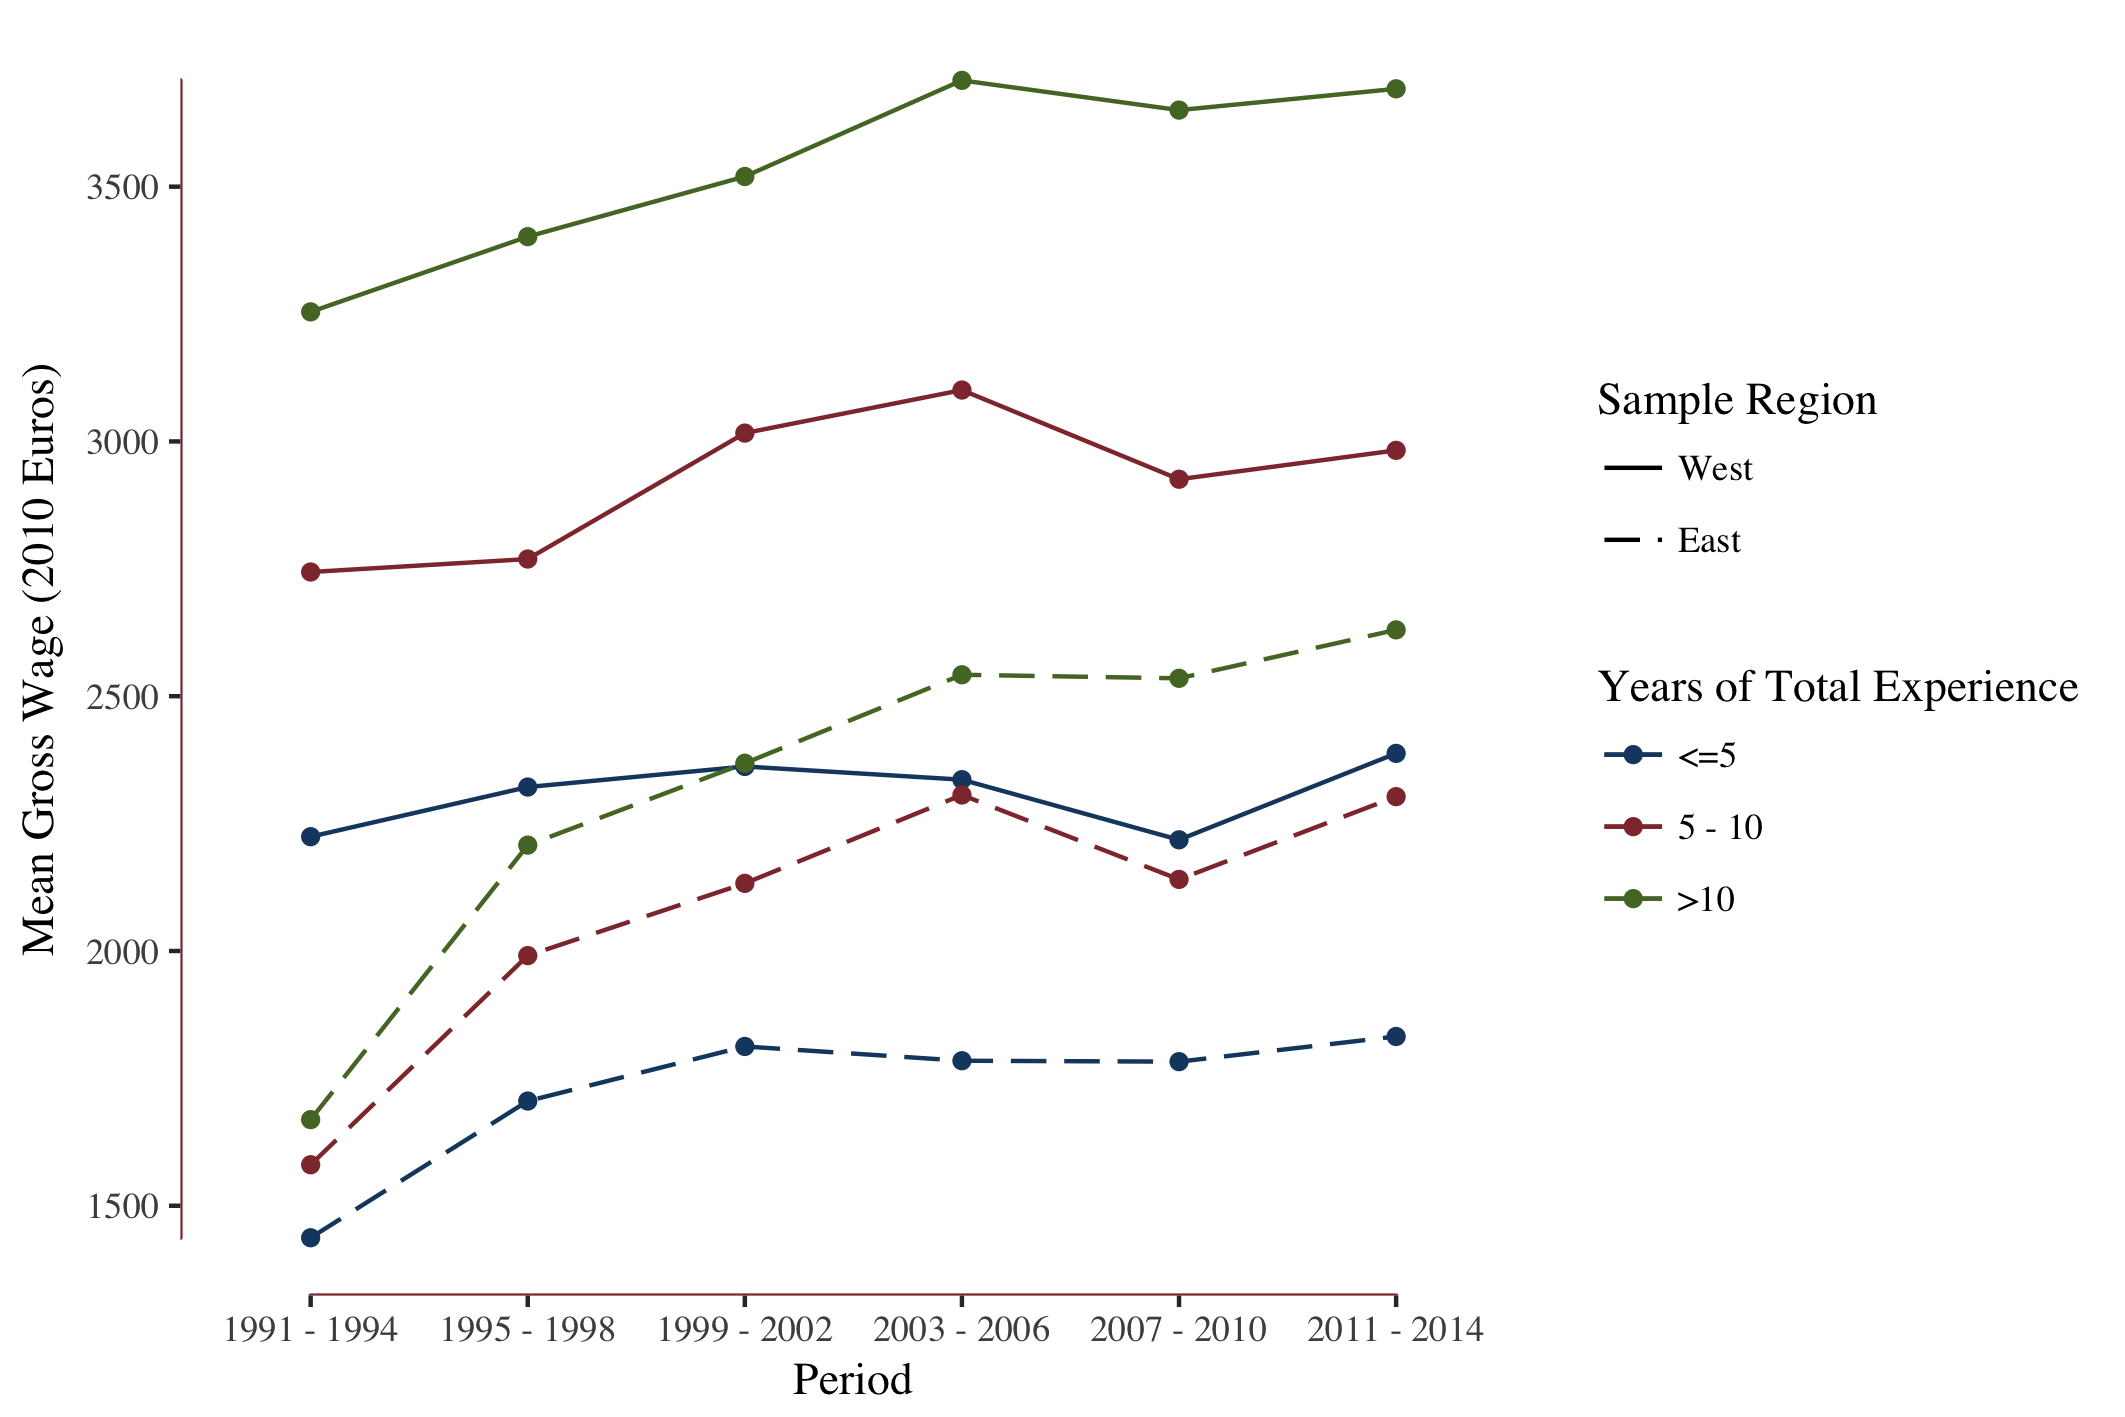
\includegraphics[width=\textwidth]{/Users/Christian/Statistik_Studium/EconProject/Code/Graphics/plotMeanWagesByTotalExp.png}
    \caption{Average Wages by Total Experience}
    \label{fig:MeanWagesByTotalExp}
\end{figure}

\begin{figure}[!h]
    \centering
    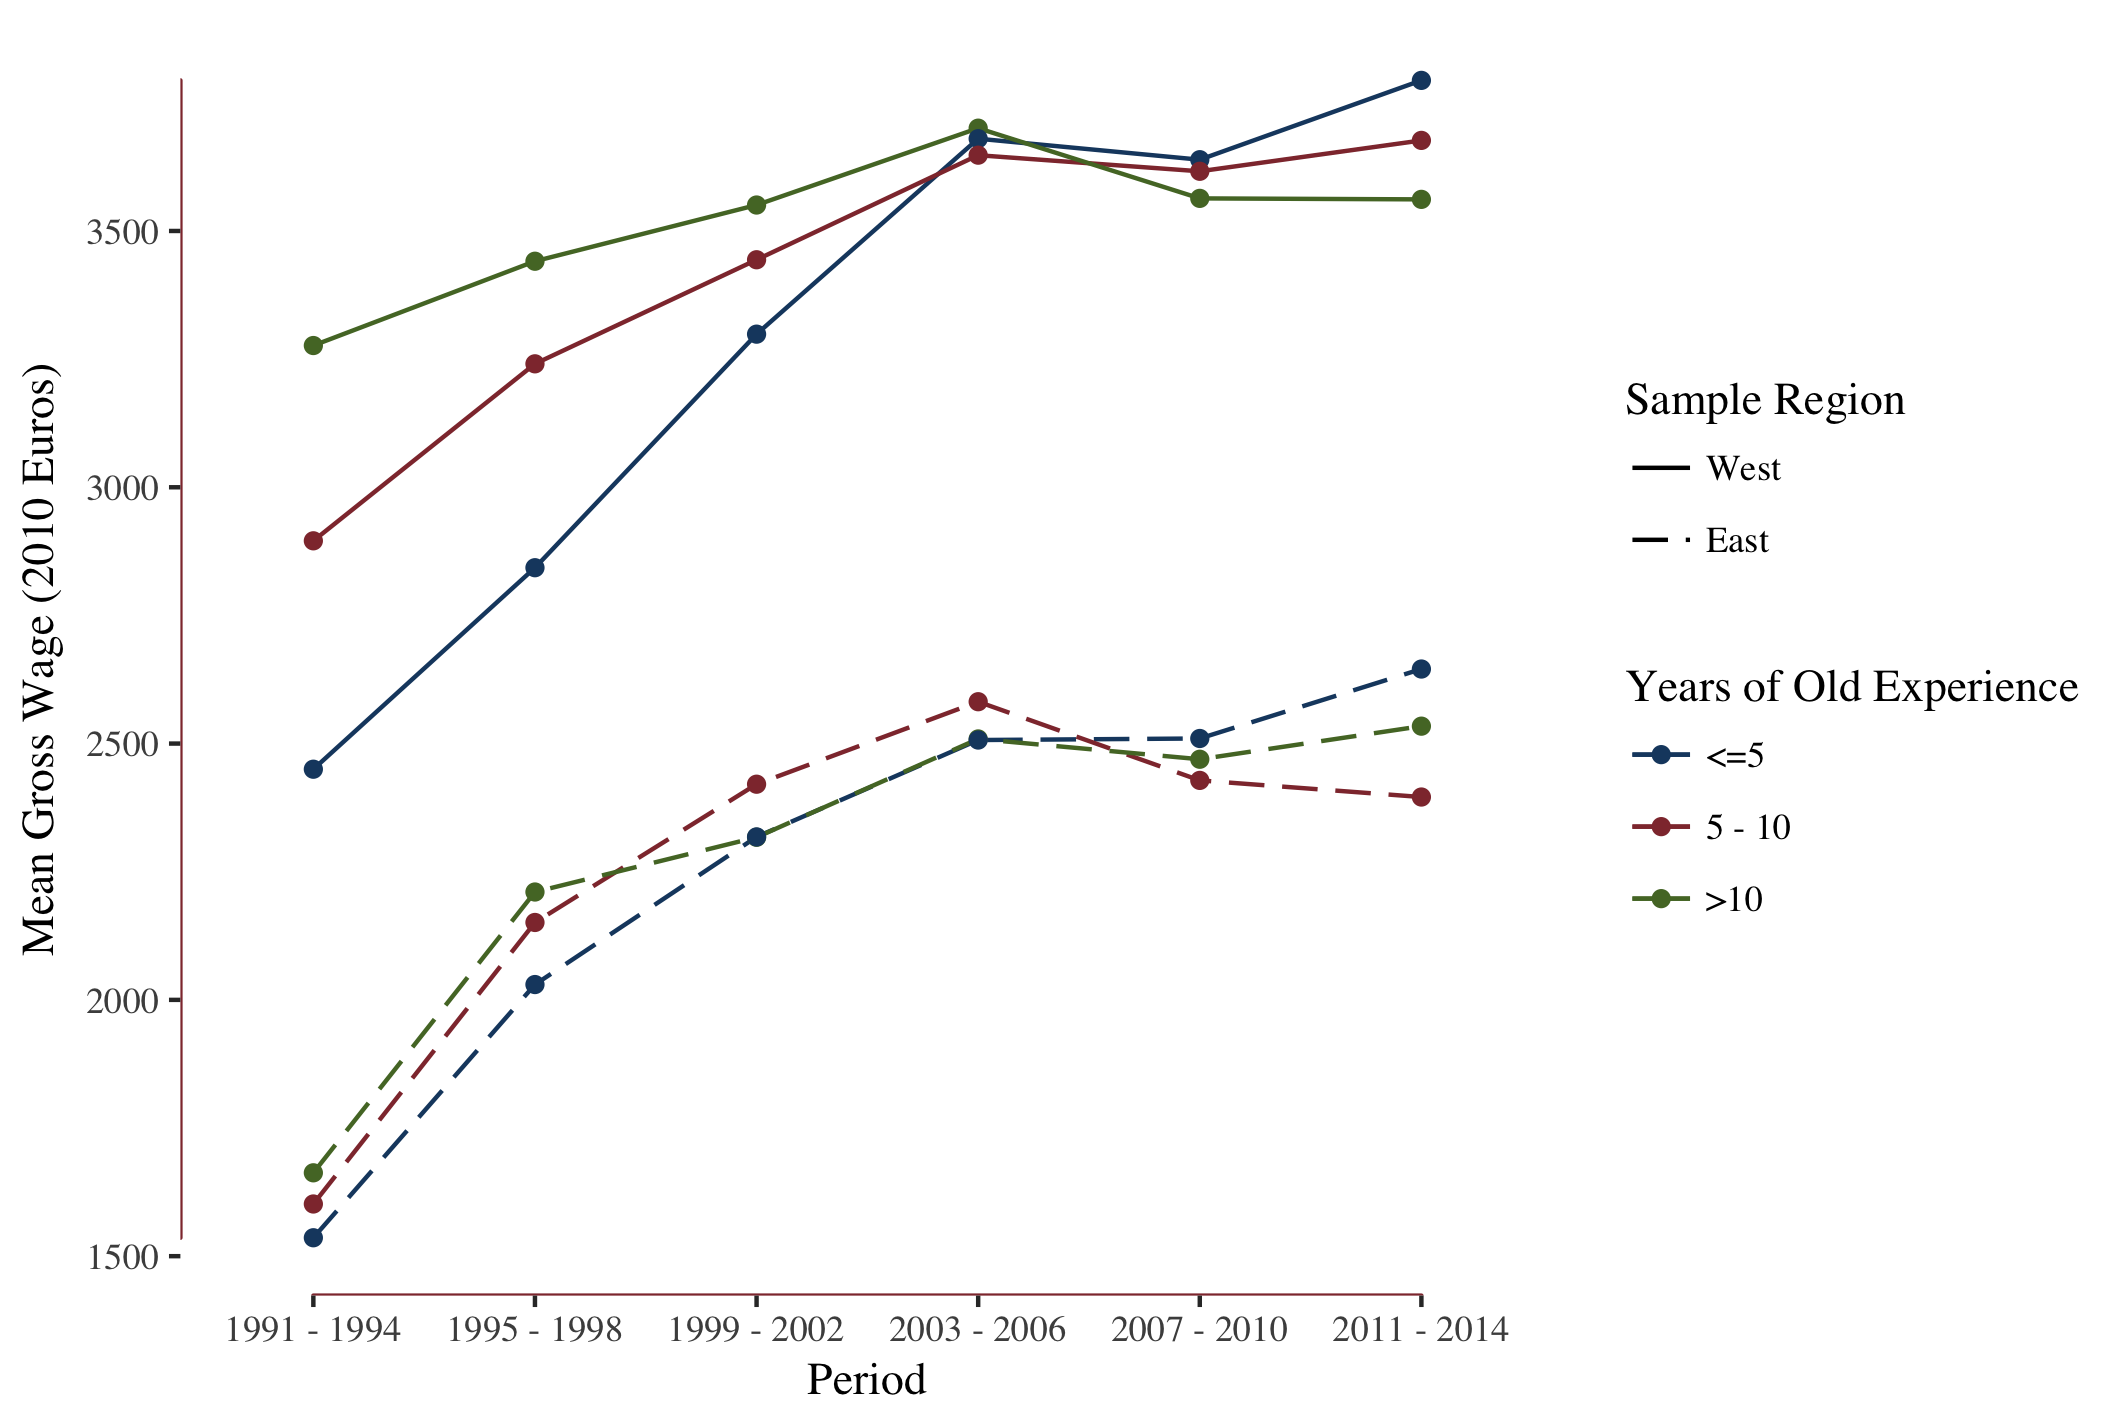
\includegraphics[width=\textwidth]{/Users/Christian/Statistik_Studium/EconProject/Code/Graphics/plotMeanWagesByOldExp.png}
    \caption{Average Wages by Old Experience}
    \label{fig:MeanWagesByOldExp}
\end{figure}

\begin{figure}[!h]
    \centering
    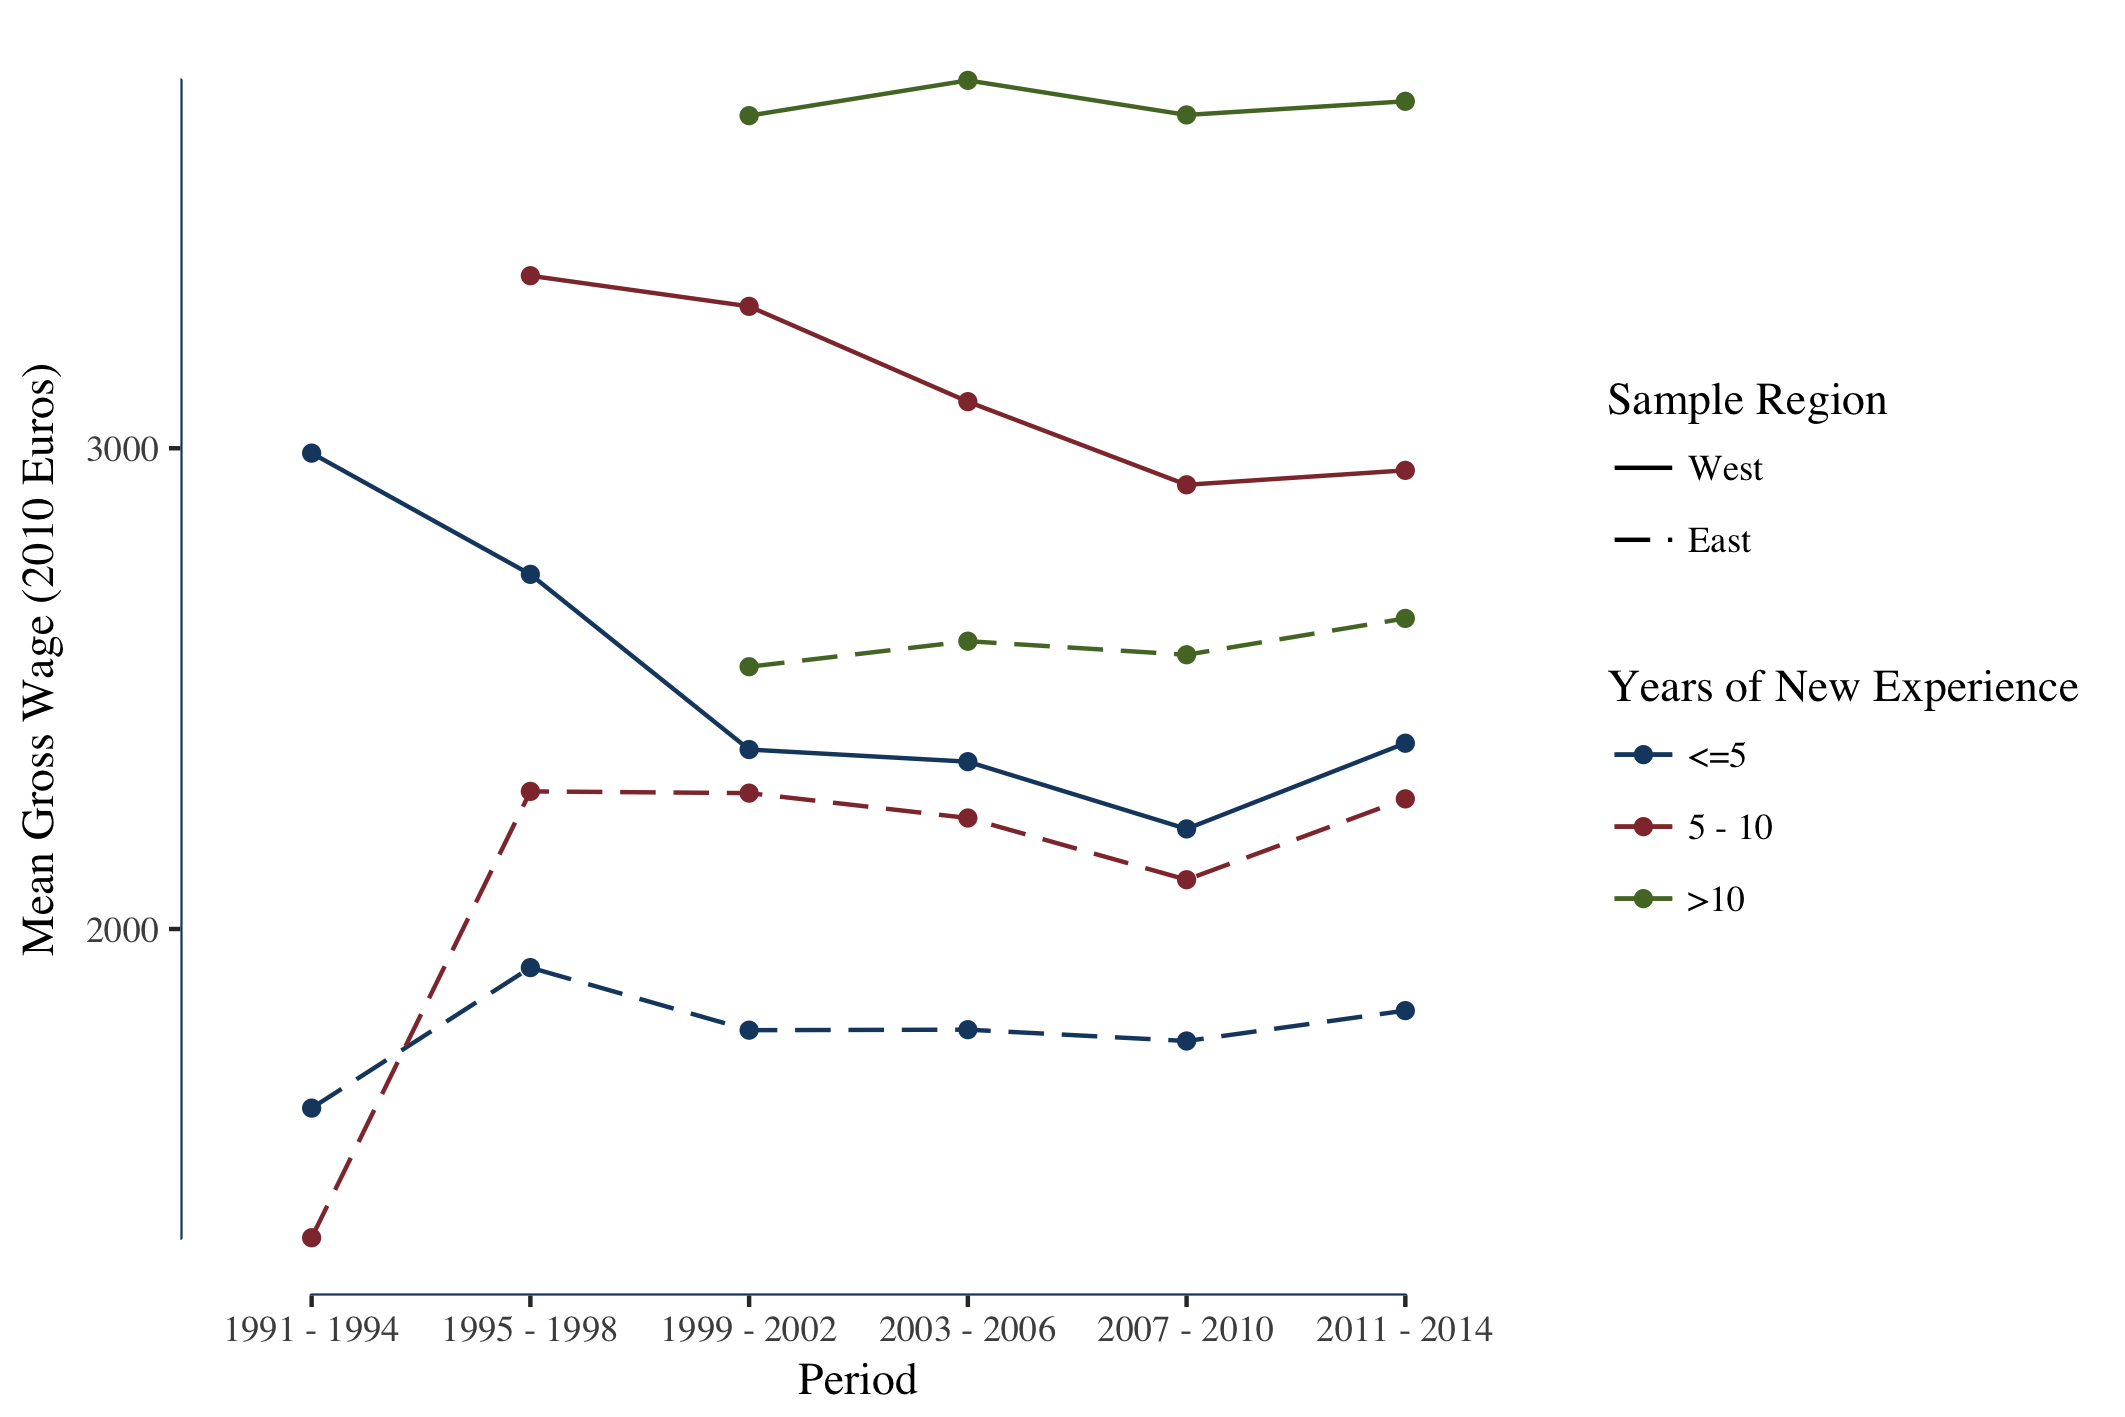
\includegraphics[width=\textwidth]{/Users/Christian/Statistik_Studium/EconProject/Code/Graphics/plotMeanWagesByNewExp.png}
    \caption{Average Wages by New Experience}
    \label{fig:MeanWagesByNewExp}
\end{figure}

\begin{figure}[!h]
    \centering
    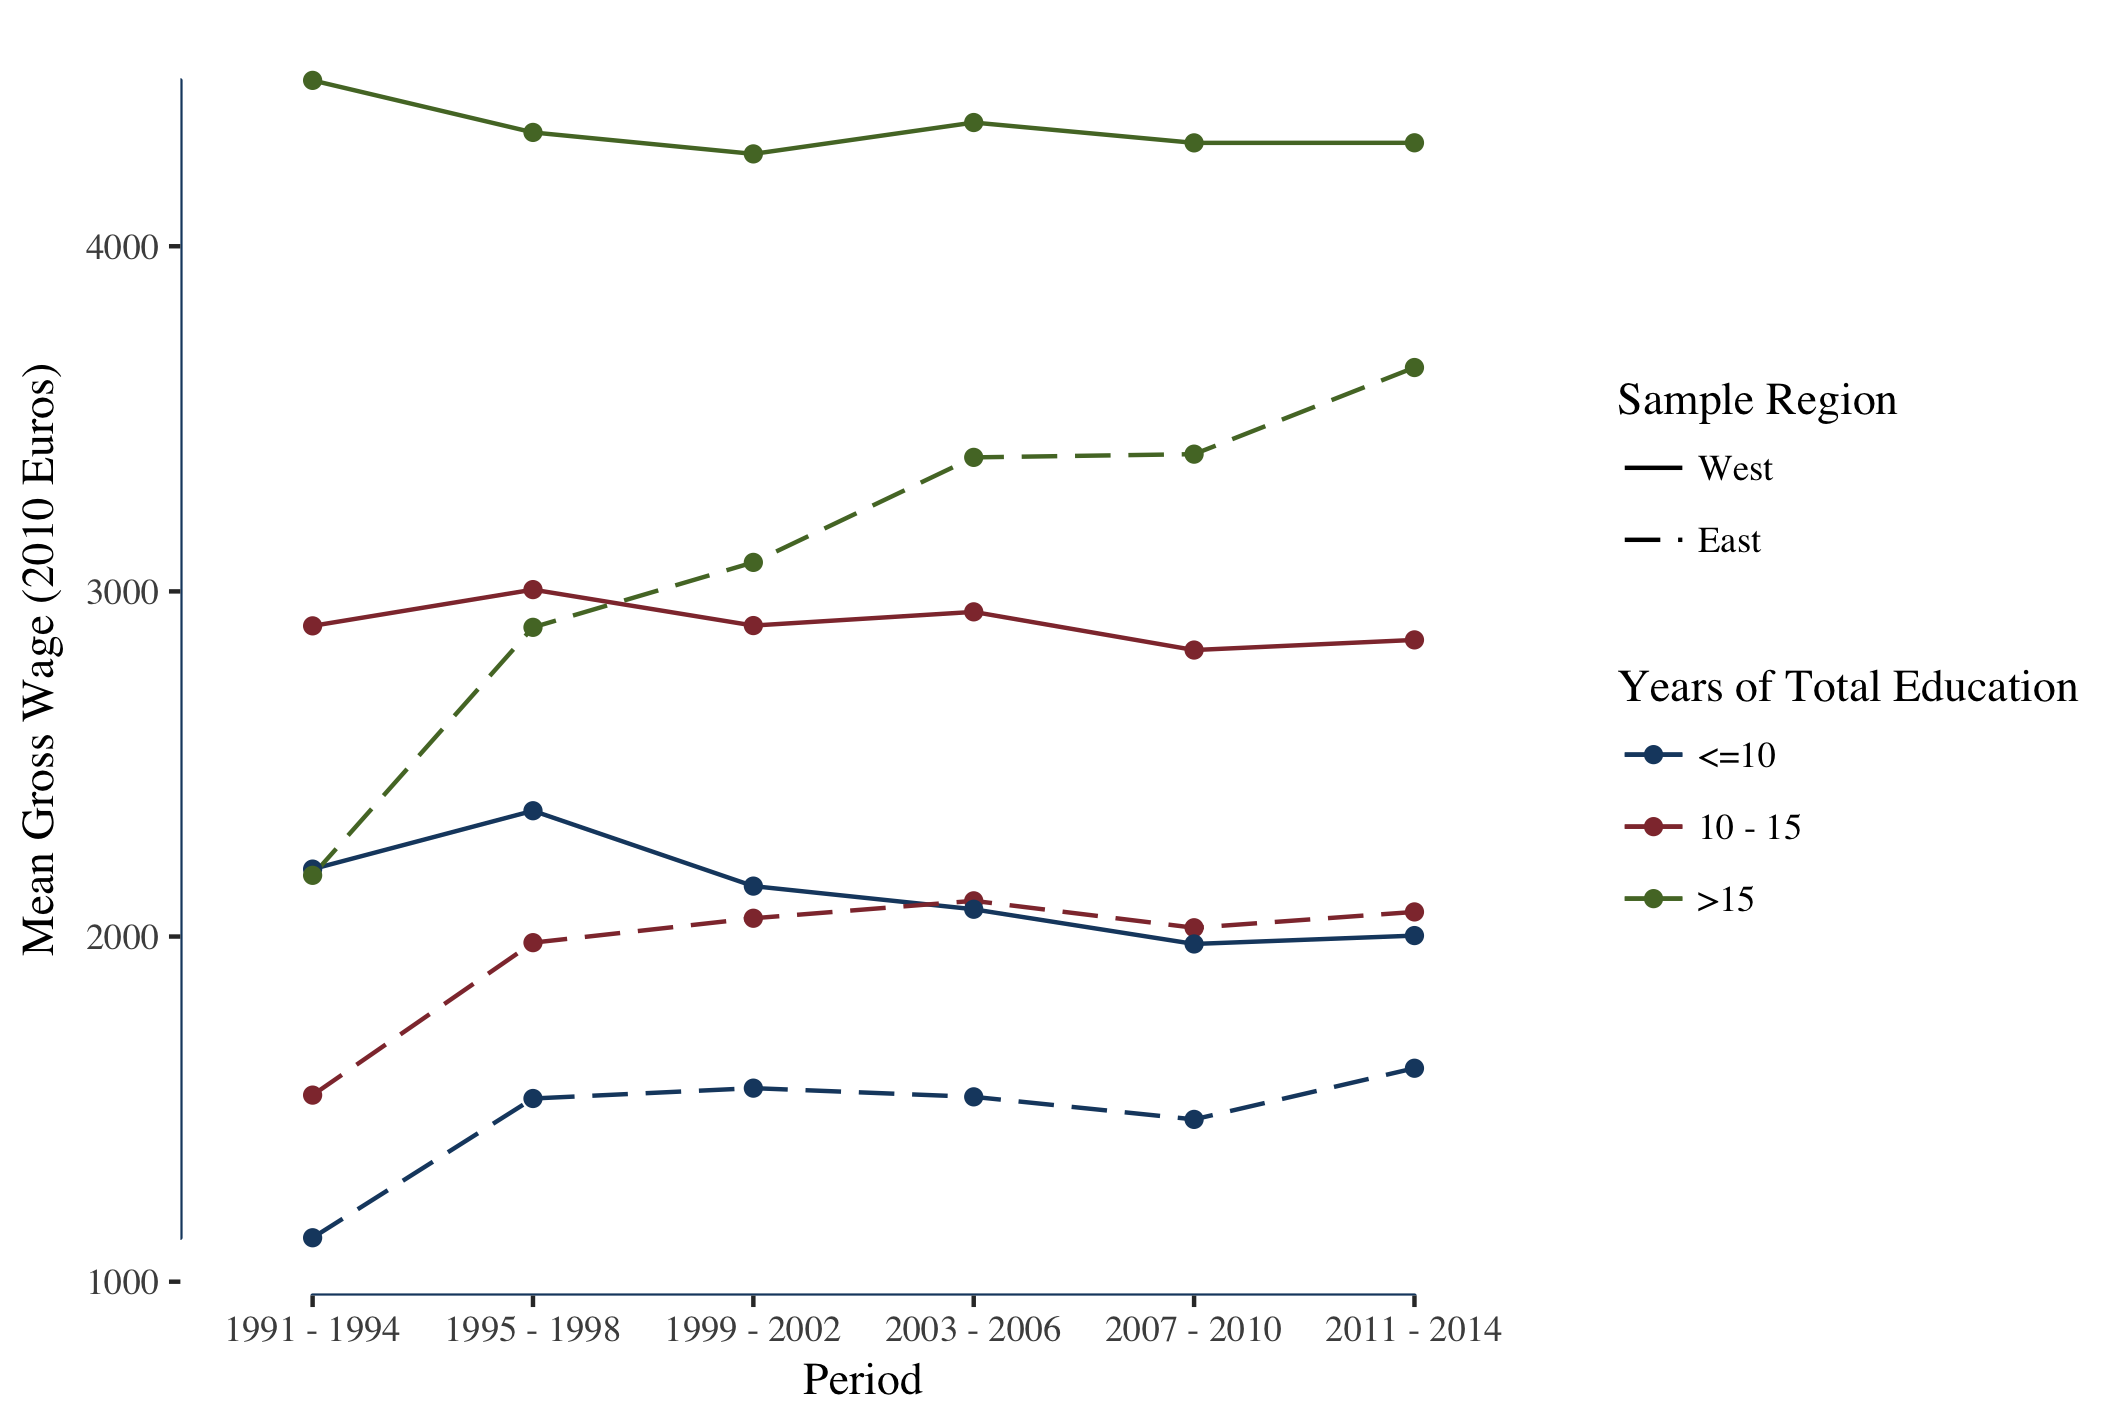
\includegraphics[width=\textwidth]{/Users/Christian/Statistik_Studium/EconProject/Code/Graphics/plotMeanWagesByTotalEdu.png}
    \caption{Average Wages by Total Education}
    \label{fig:MeanWagesByTotalEdu}
\end{figure}

\begin{figure}[!h]
    \centering
    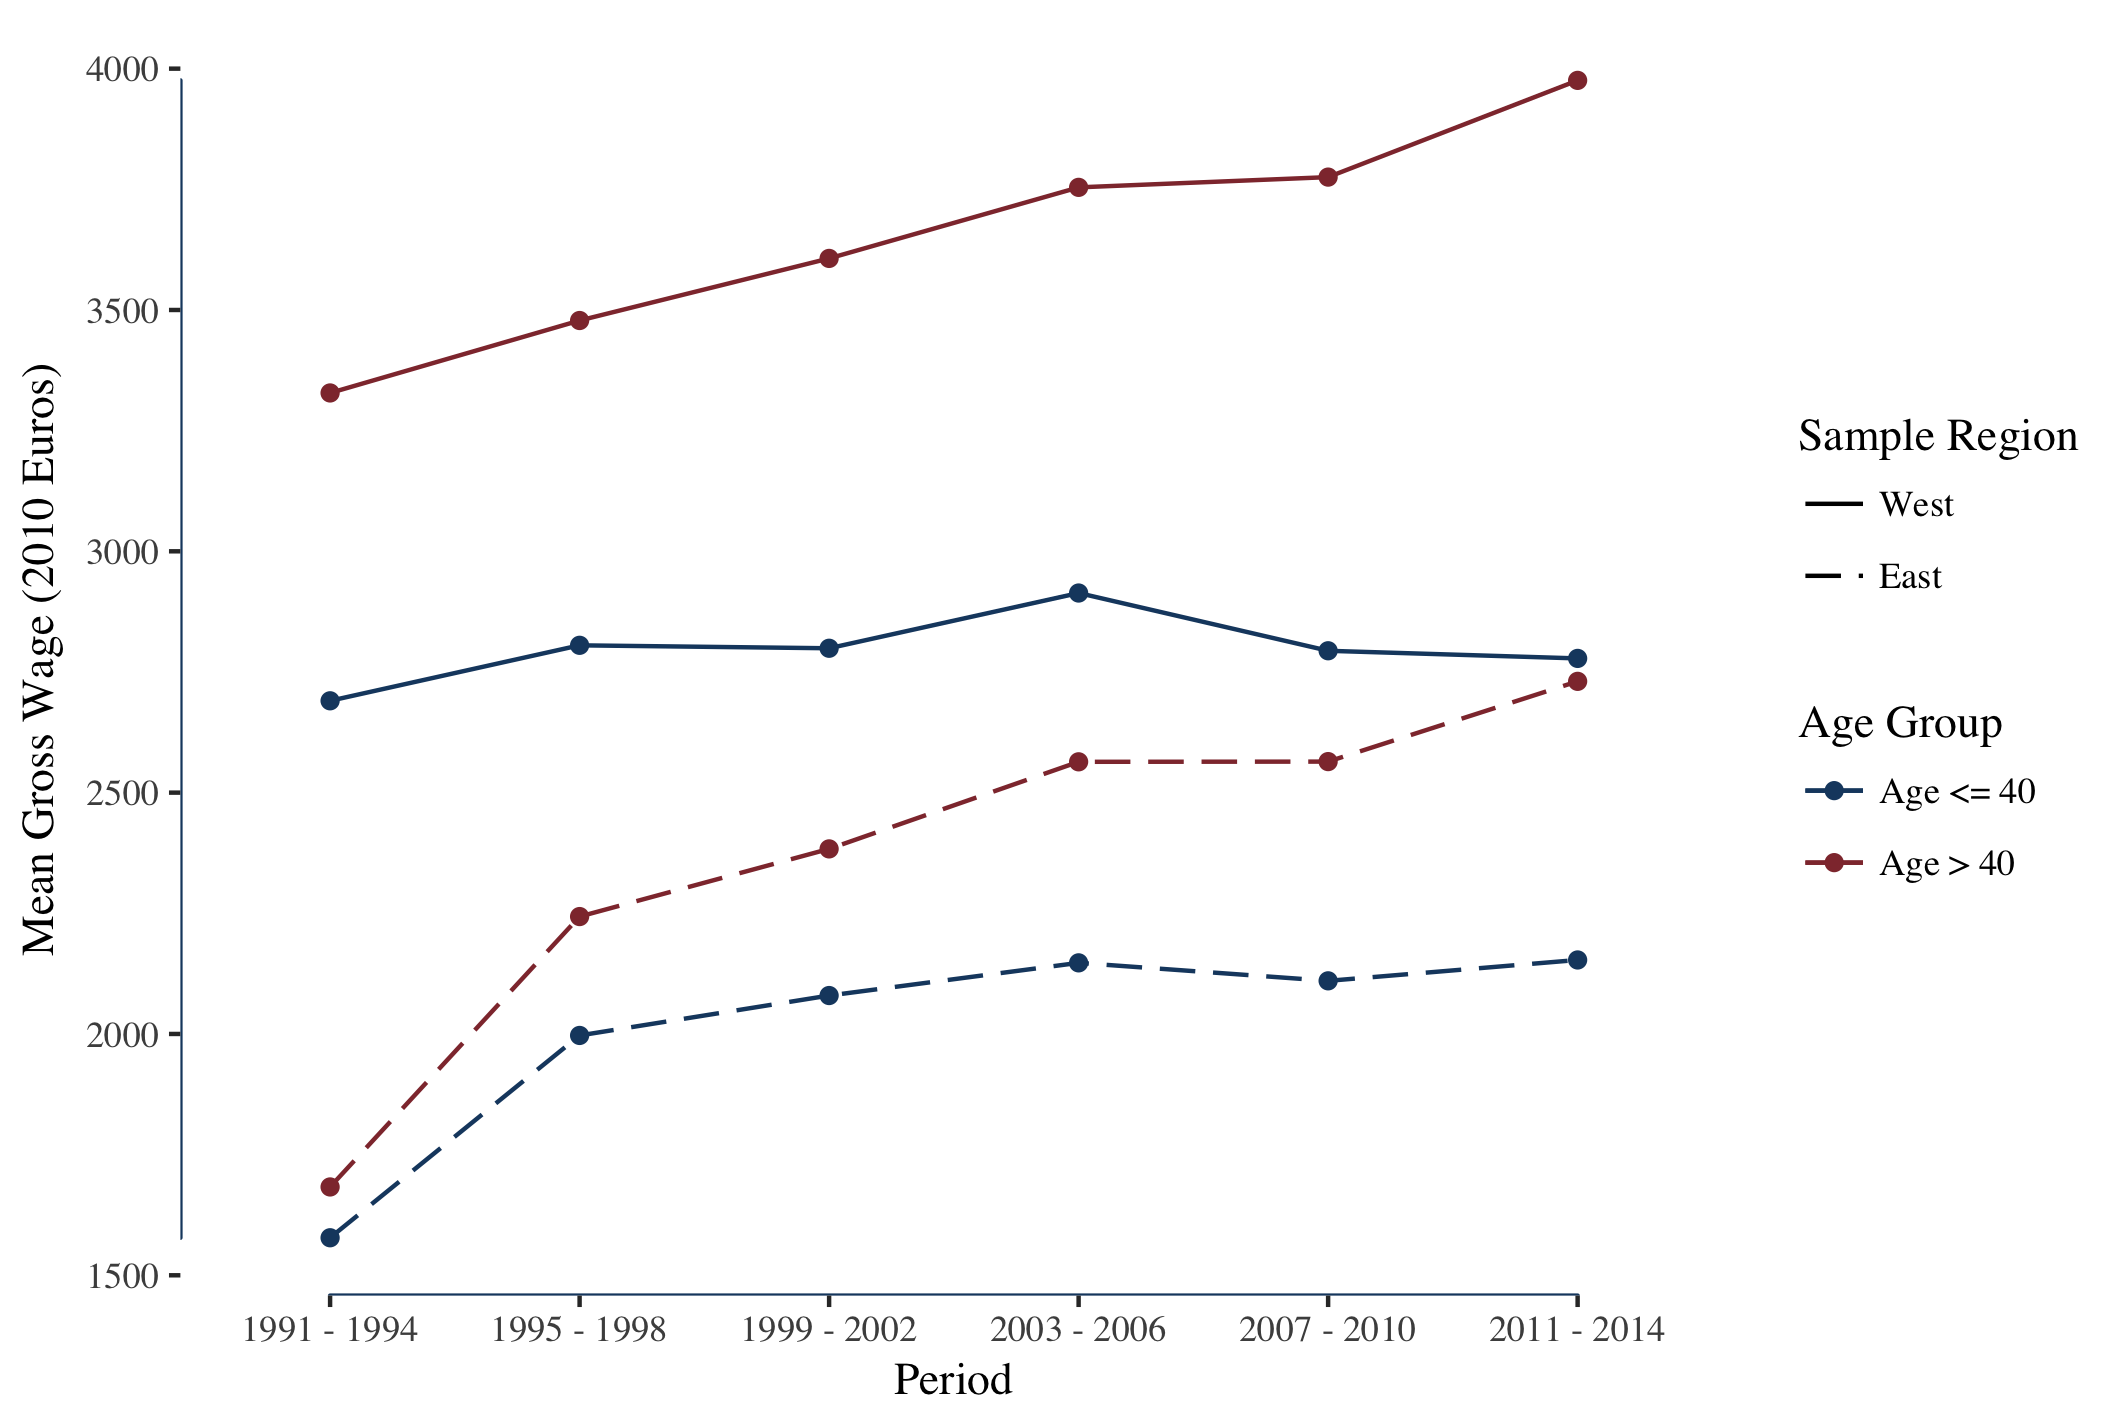
\includegraphics[width=\textwidth]{/Users/Christian/Statistik_Studium/EconProject/Code/Graphics/plotMeanWagesByAgeGroup.png}
    \caption{Average Wages by Age Group}
    \label{fig:MeanWagesByAgeGroup}
\end{figure}

\begin{figure}[!h]
    \centering
    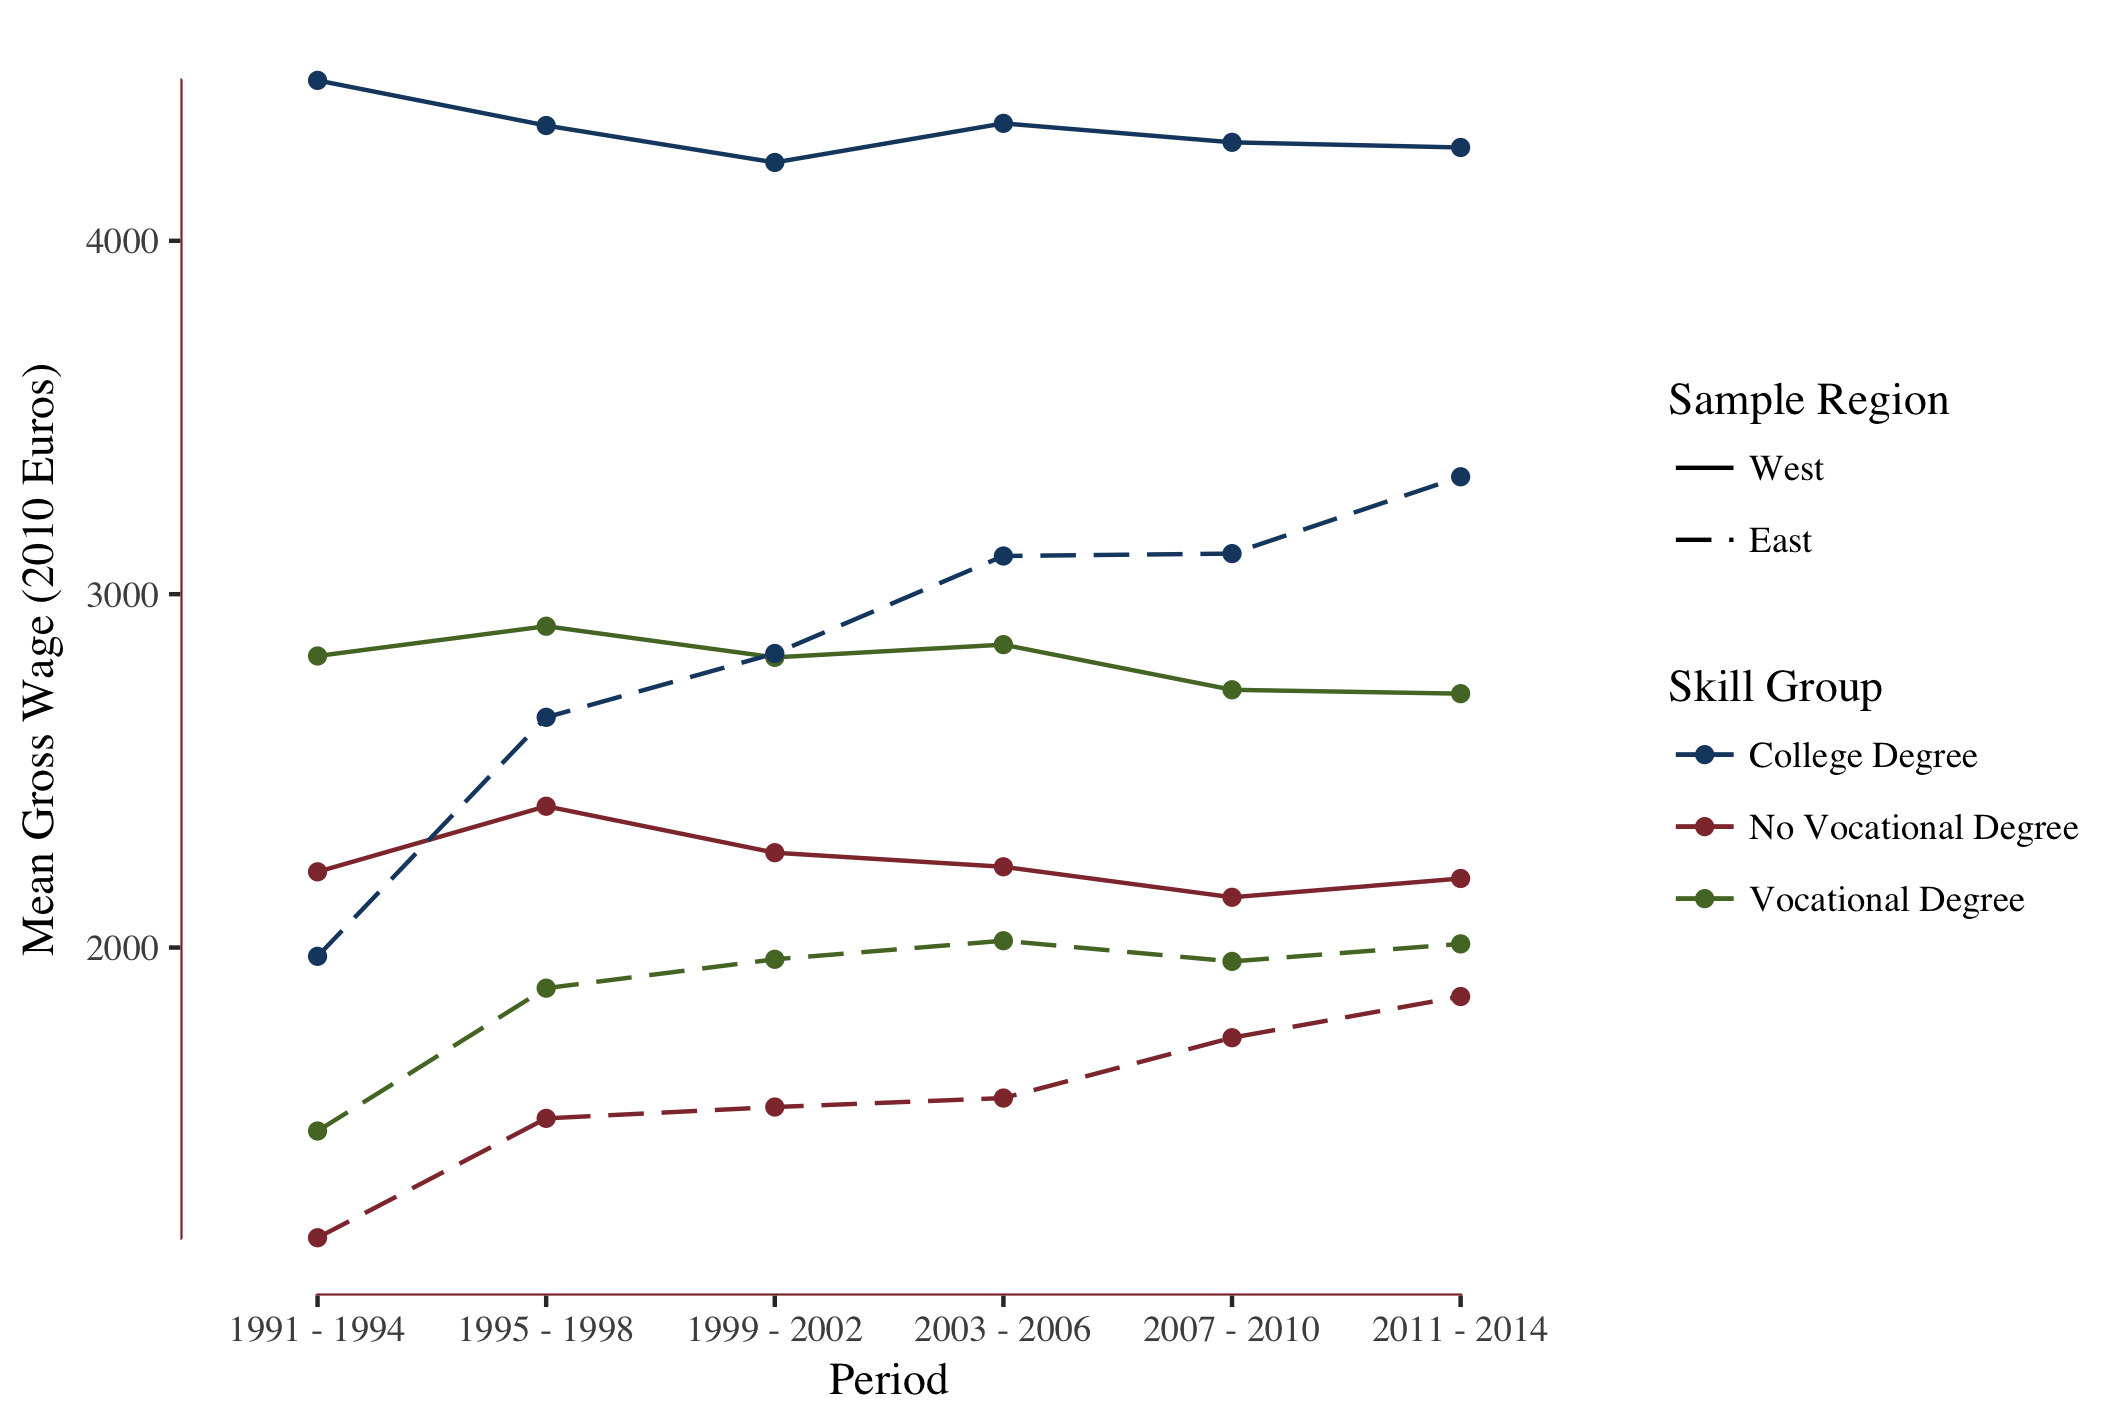
\includegraphics[width=\textwidth]{/Users/Christian/Statistik_Studium/EconProject/Code/Graphics/plotMeanWagesBySkillGroup.png}
    \caption{Average Wages by Skill Group}
    \label{fig:MeanWagesBySkillGroup}
\end{figure}

\FloatBarrier
\subsection{Distribution of Explanatory Variables}
Regarding the distribution of experience and education in the sub-samples one can draw the following conclusions from the graphs below:
\begin{enumerate}
	\item Overall levels of Experience are relatively constant in East Germany while they are decreasing over time in the West. This seems to be due both to the quicker fall in Old Experience in the West as well as the faster rise in New Experience in the East (see Figure \ref{fig:MeanExp}).
	\item Whereas the regional differences in experience levels seem to disappear over time in the young sample they tend to increase in the sample of old individuals(see Figure \ref{fig:MeanExpByAgeGroup}). This might suggest some kind of selection affect or different sample attrition.
	\item East German college graduates have significantly more experience than their West German peers whereas this relation is turned the other way around when looking at individuals without vocational degree. For Individuals with a vocational Degree experience levels are virtually the same across regions(see Figure \ref{fig:MeanExpBySkillGroup}).
	\item Levels of Total Education are very similar across regions, while the share of New Education is considerably higher in West Germany throughout the time frame (see Figure \ref{fig:MeanEdu}). This seems to hold for both age group sub-samples (see Figure \ref{fig:MeanEduByAgeGroup}).
	\item Overall there is a slight rise in the mean years of Total Education. Mean years of Old and New Education converge towards each other. Overall the share of Old Education is higher in the East. (see Figure \ref{fig:MeanEdu}. This seems to be the case in both age groups (see Figure \ref{fig:MeanEduByAgeGroup}).
\end{enumerate}
\begin{figure}[!h]
    \centering
    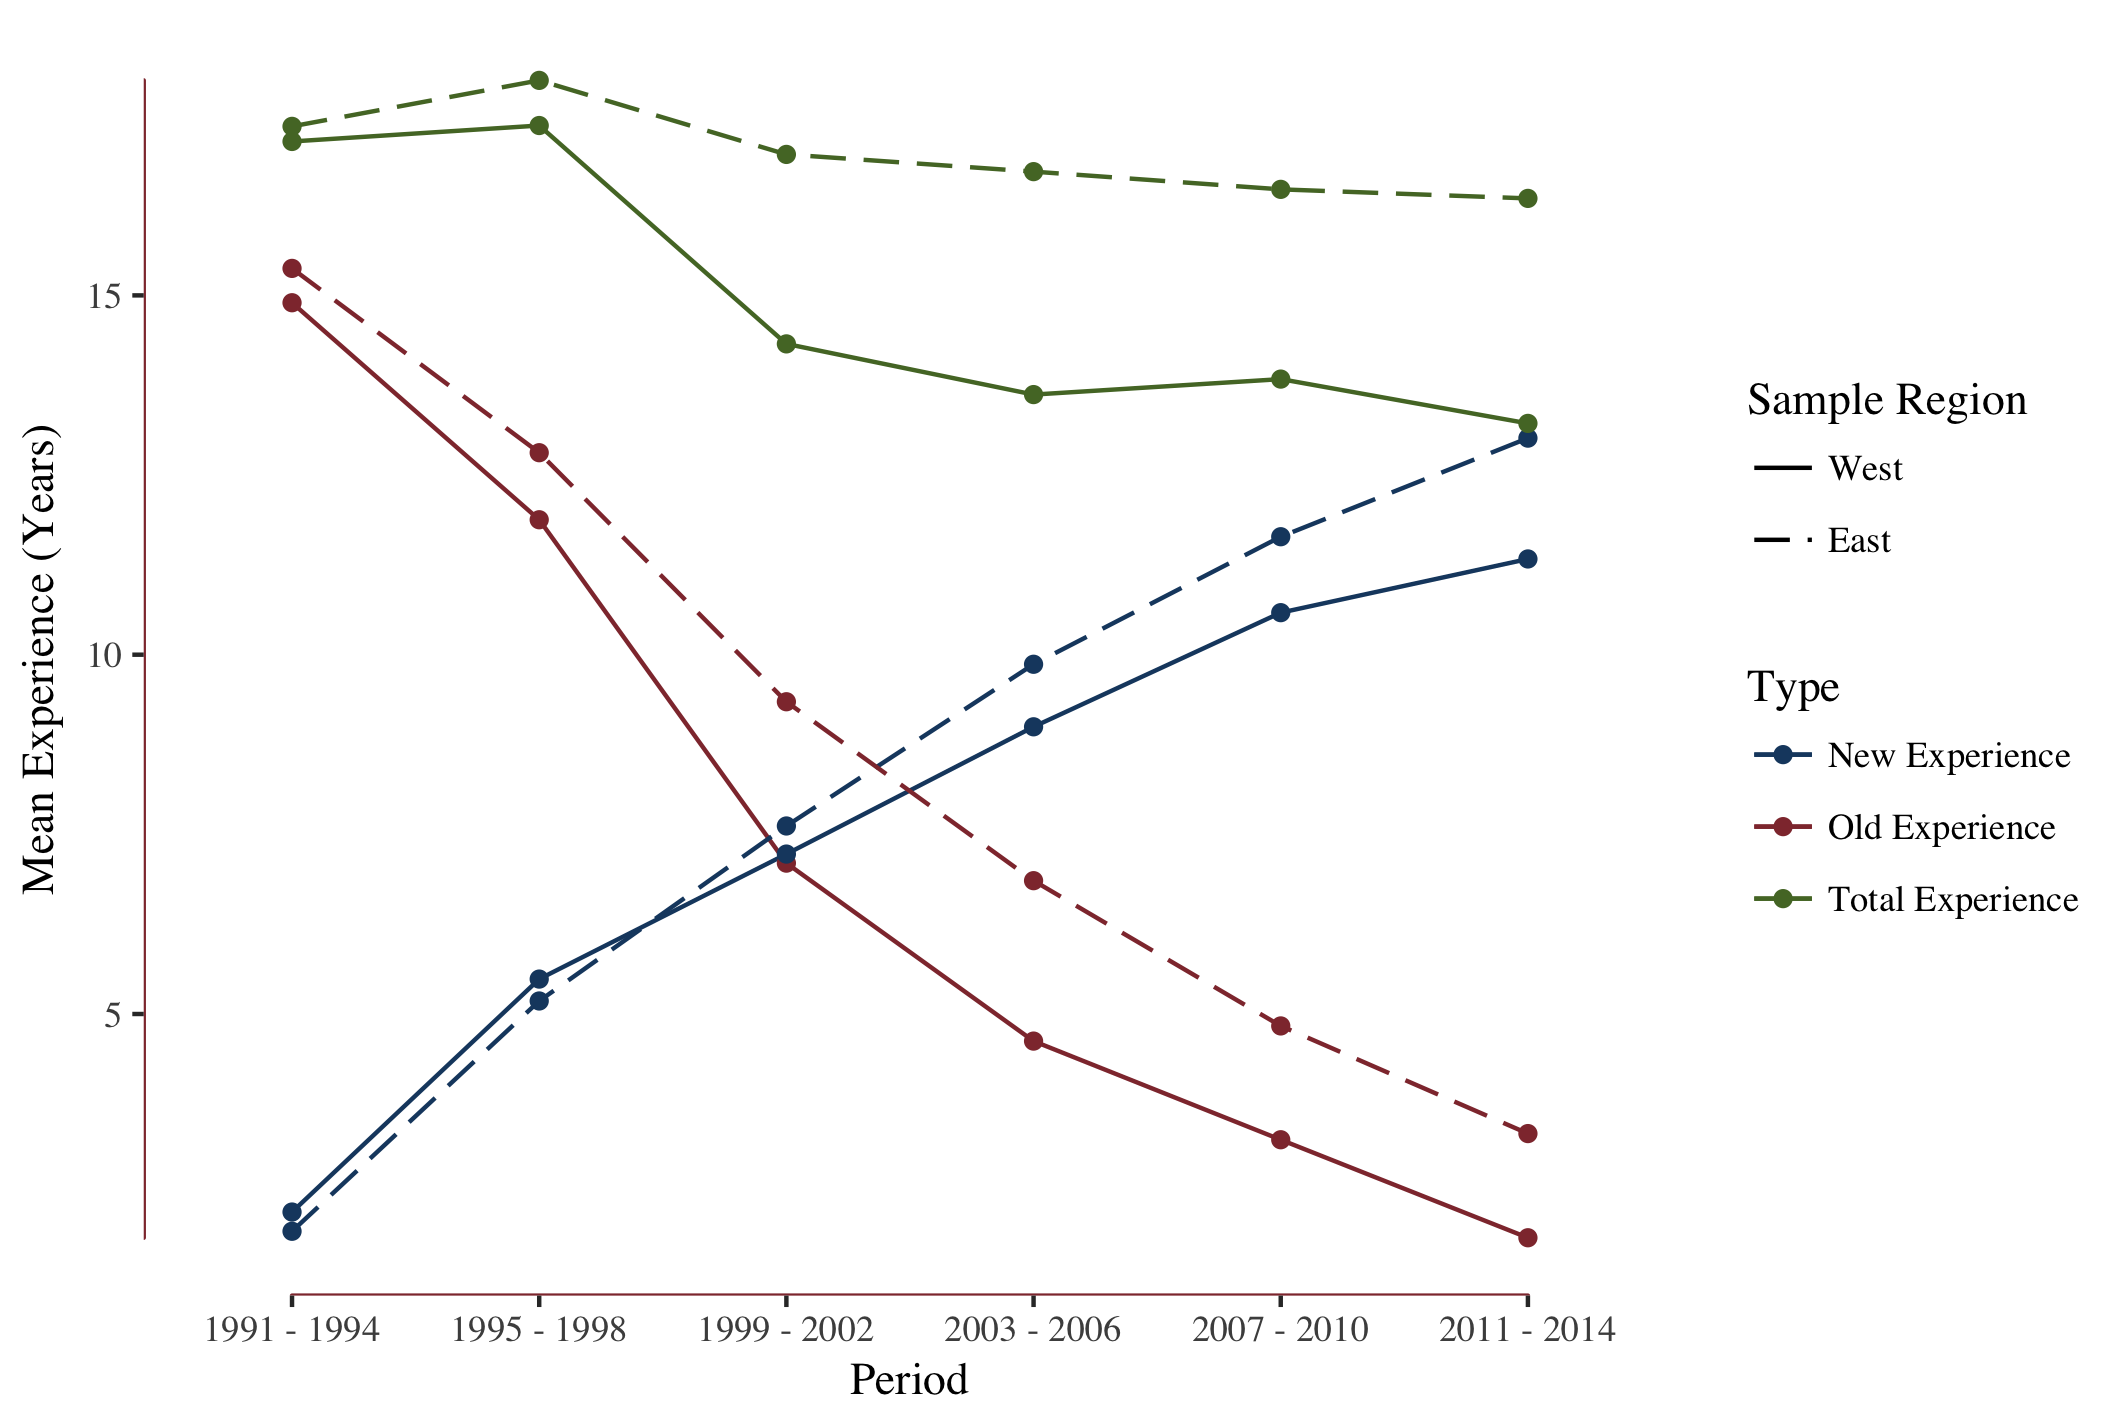
\includegraphics[width=\textwidth]{/Users/Christian/Statistik_Studium/EconProject/Code/Graphics/plotMeanExp.png}
    \caption{Average Years of Experience}
    \label{fig:MeanExp}
\end{figure}

\begin{figure}[!h]
    \centering
    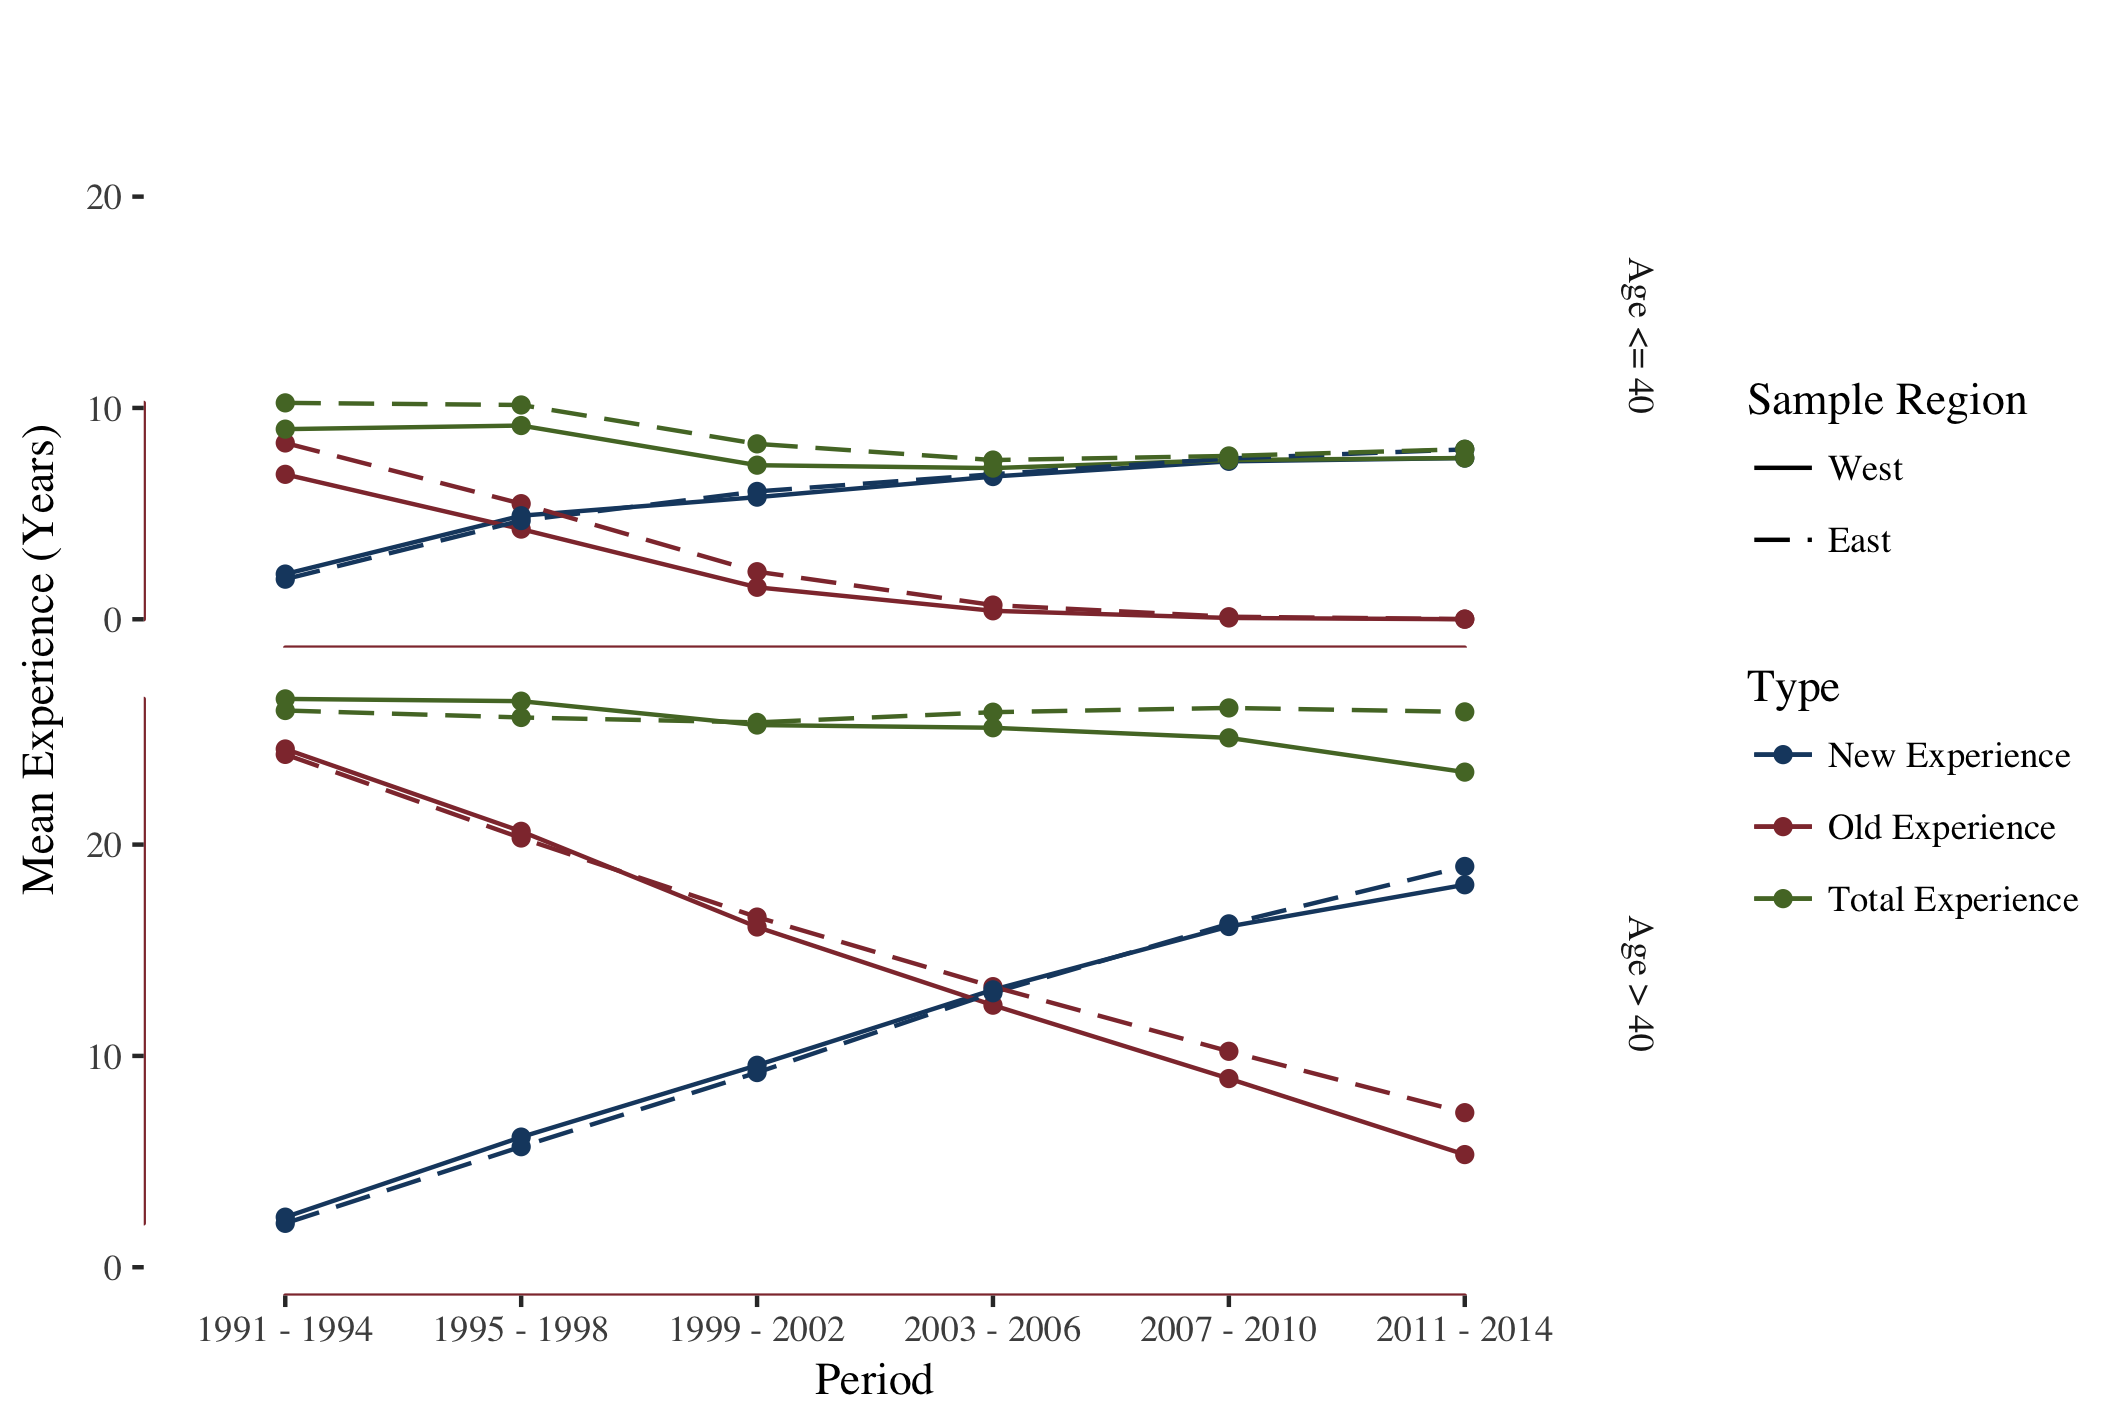
\includegraphics[width=\textwidth]{/Users/Christian/Statistik_Studium/EconProject/Code/Graphics/plotMeanExpByAgeGroup.png}
    \caption{Average Years of Experience for two Age Groups}
    \label{fig:MeanExpByAgeGroup}
\end{figure}

\begin{figure}[!h]
    \centering
    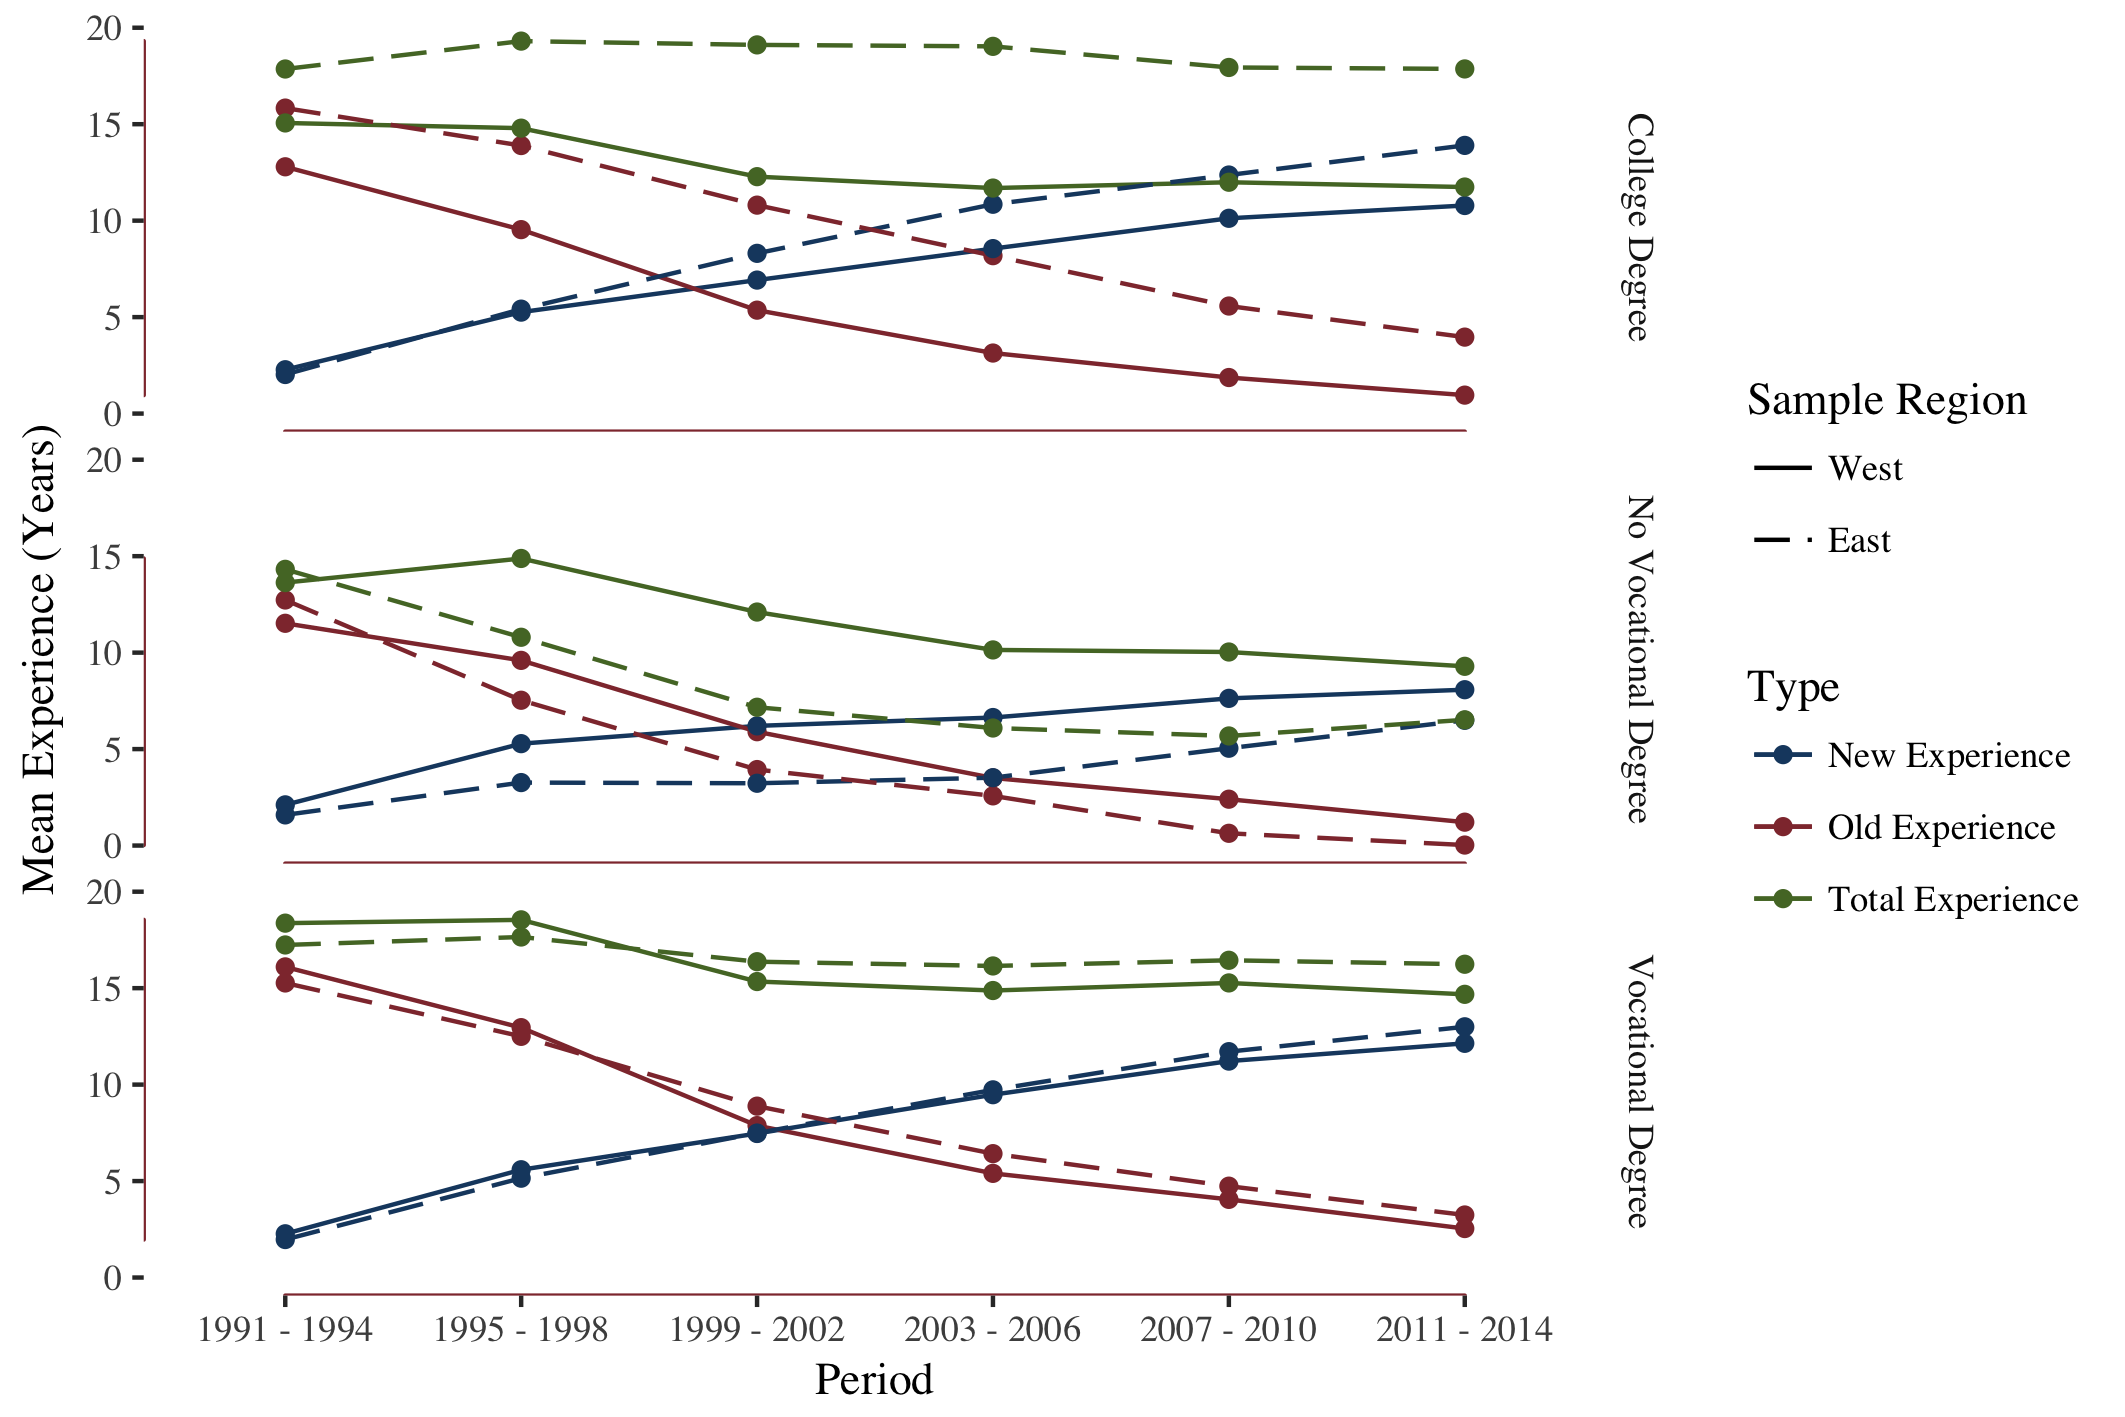
\includegraphics[width=\textwidth]{/Users/Christian/Statistik_Studium/EconProject/Code/Graphics/plotMeanExpBySkillGroup.png}
    \caption{Average Years of Experience for three Skill Groups}
    \label{fig:MeanExpBySkillGroup}
\end{figure}

\begin{figure}[!h]
    \centering
    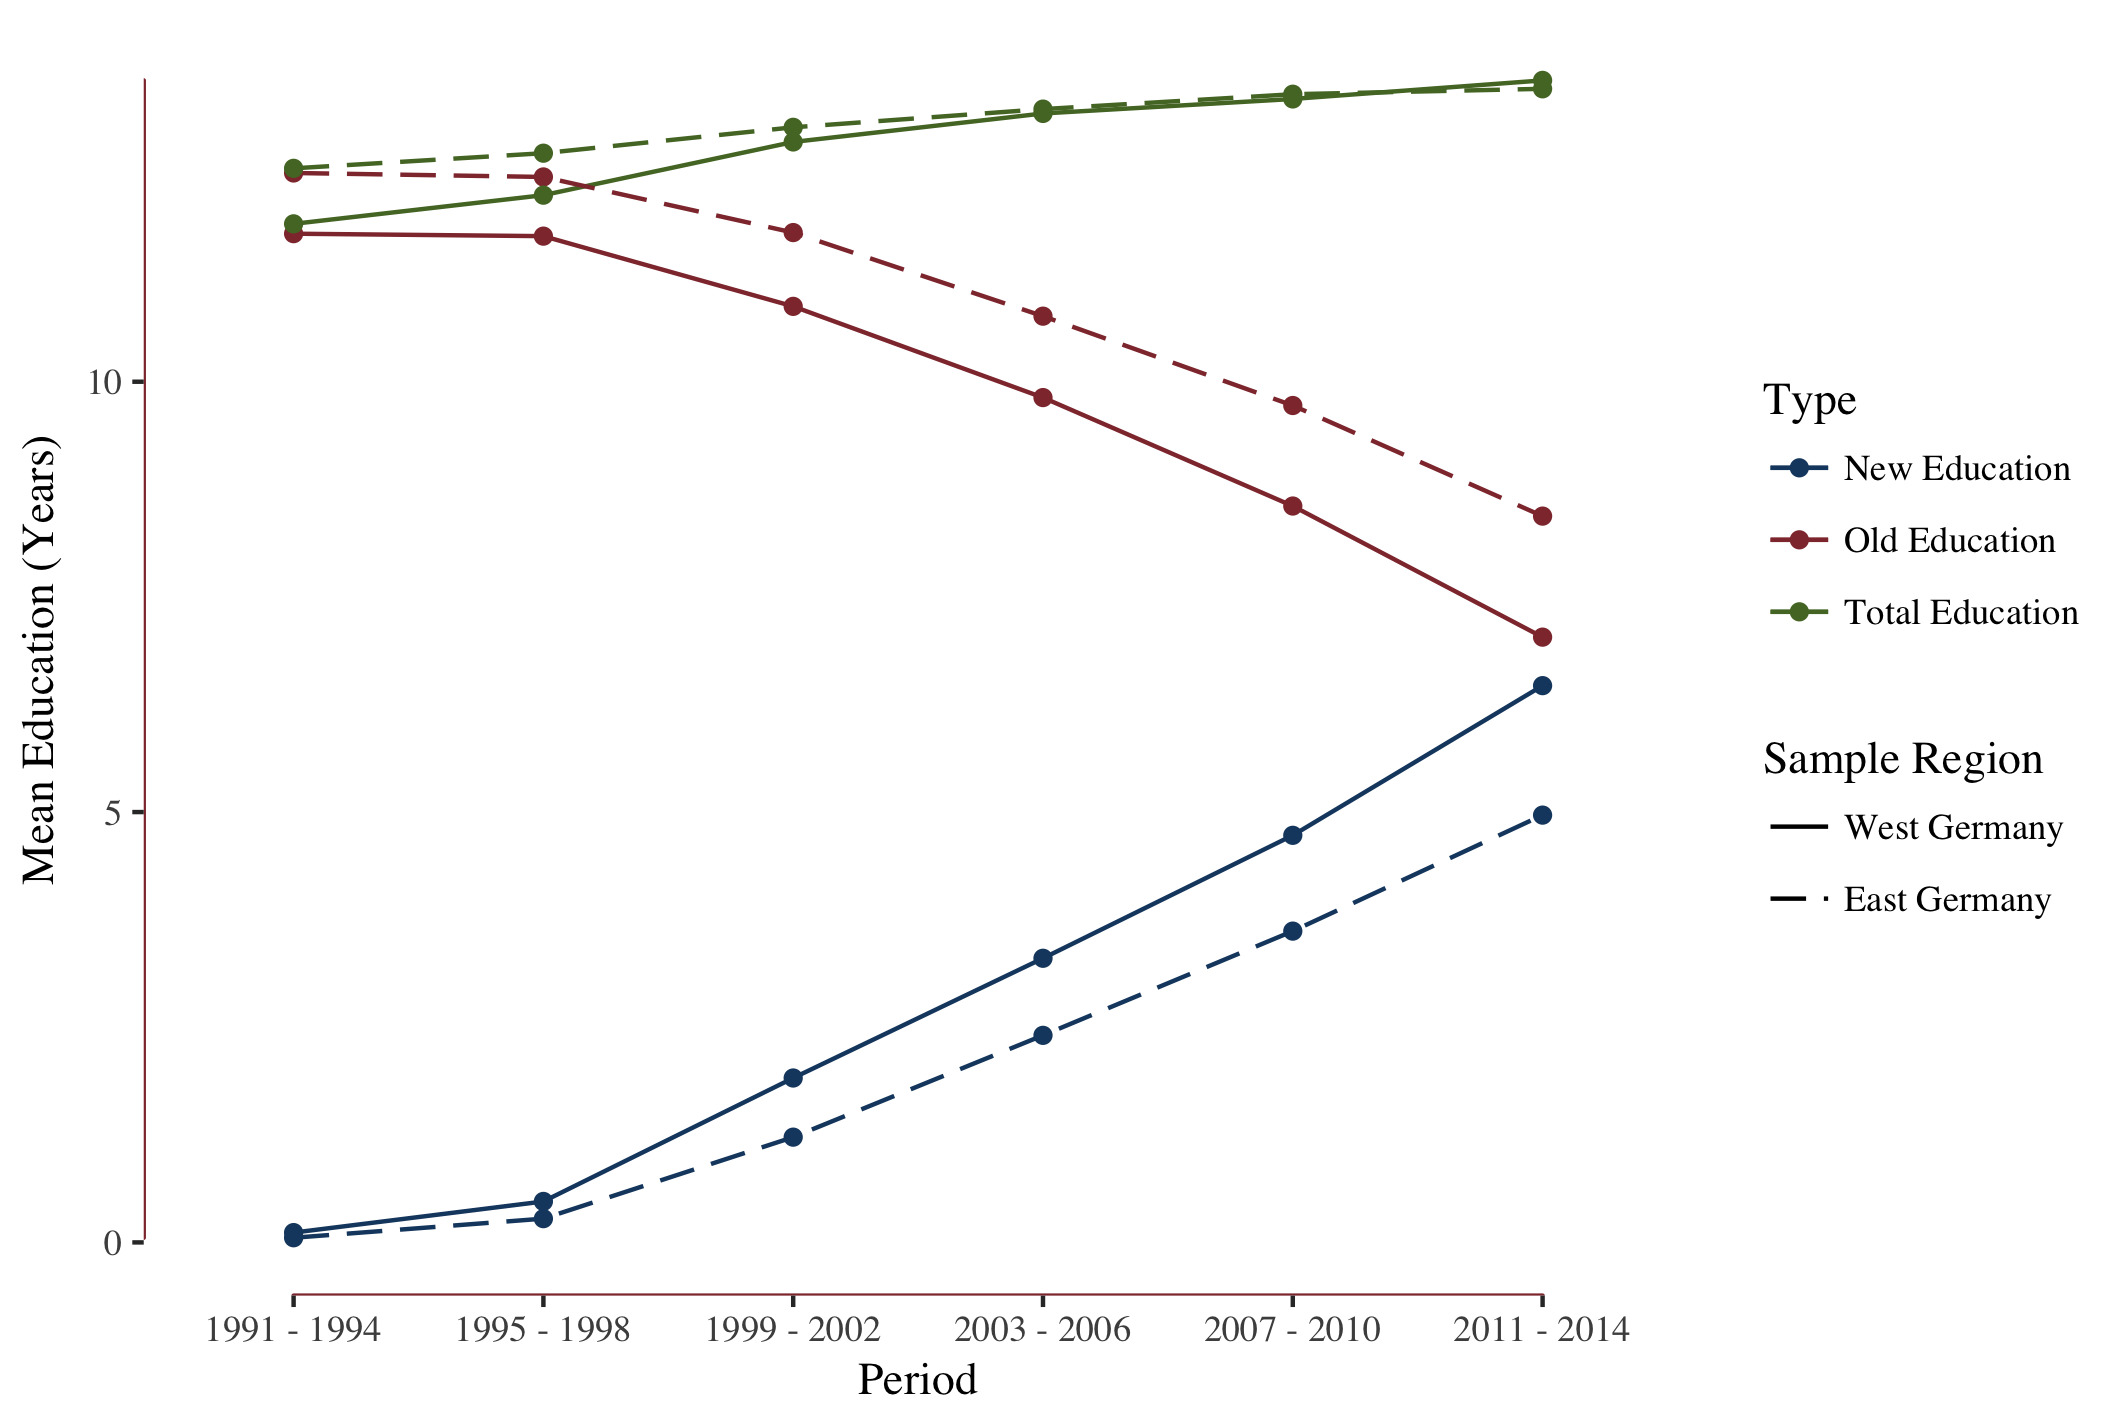
\includegraphics[width=\textwidth]{/Users/Christian/Statistik_Studium/EconProject/Code/Graphics/plotMeanEdu.png}
    \caption{Average Years of Education}
    \label{fig:MeanEdu}
\end{figure}

\begin{figure}[!h]
    \centering
    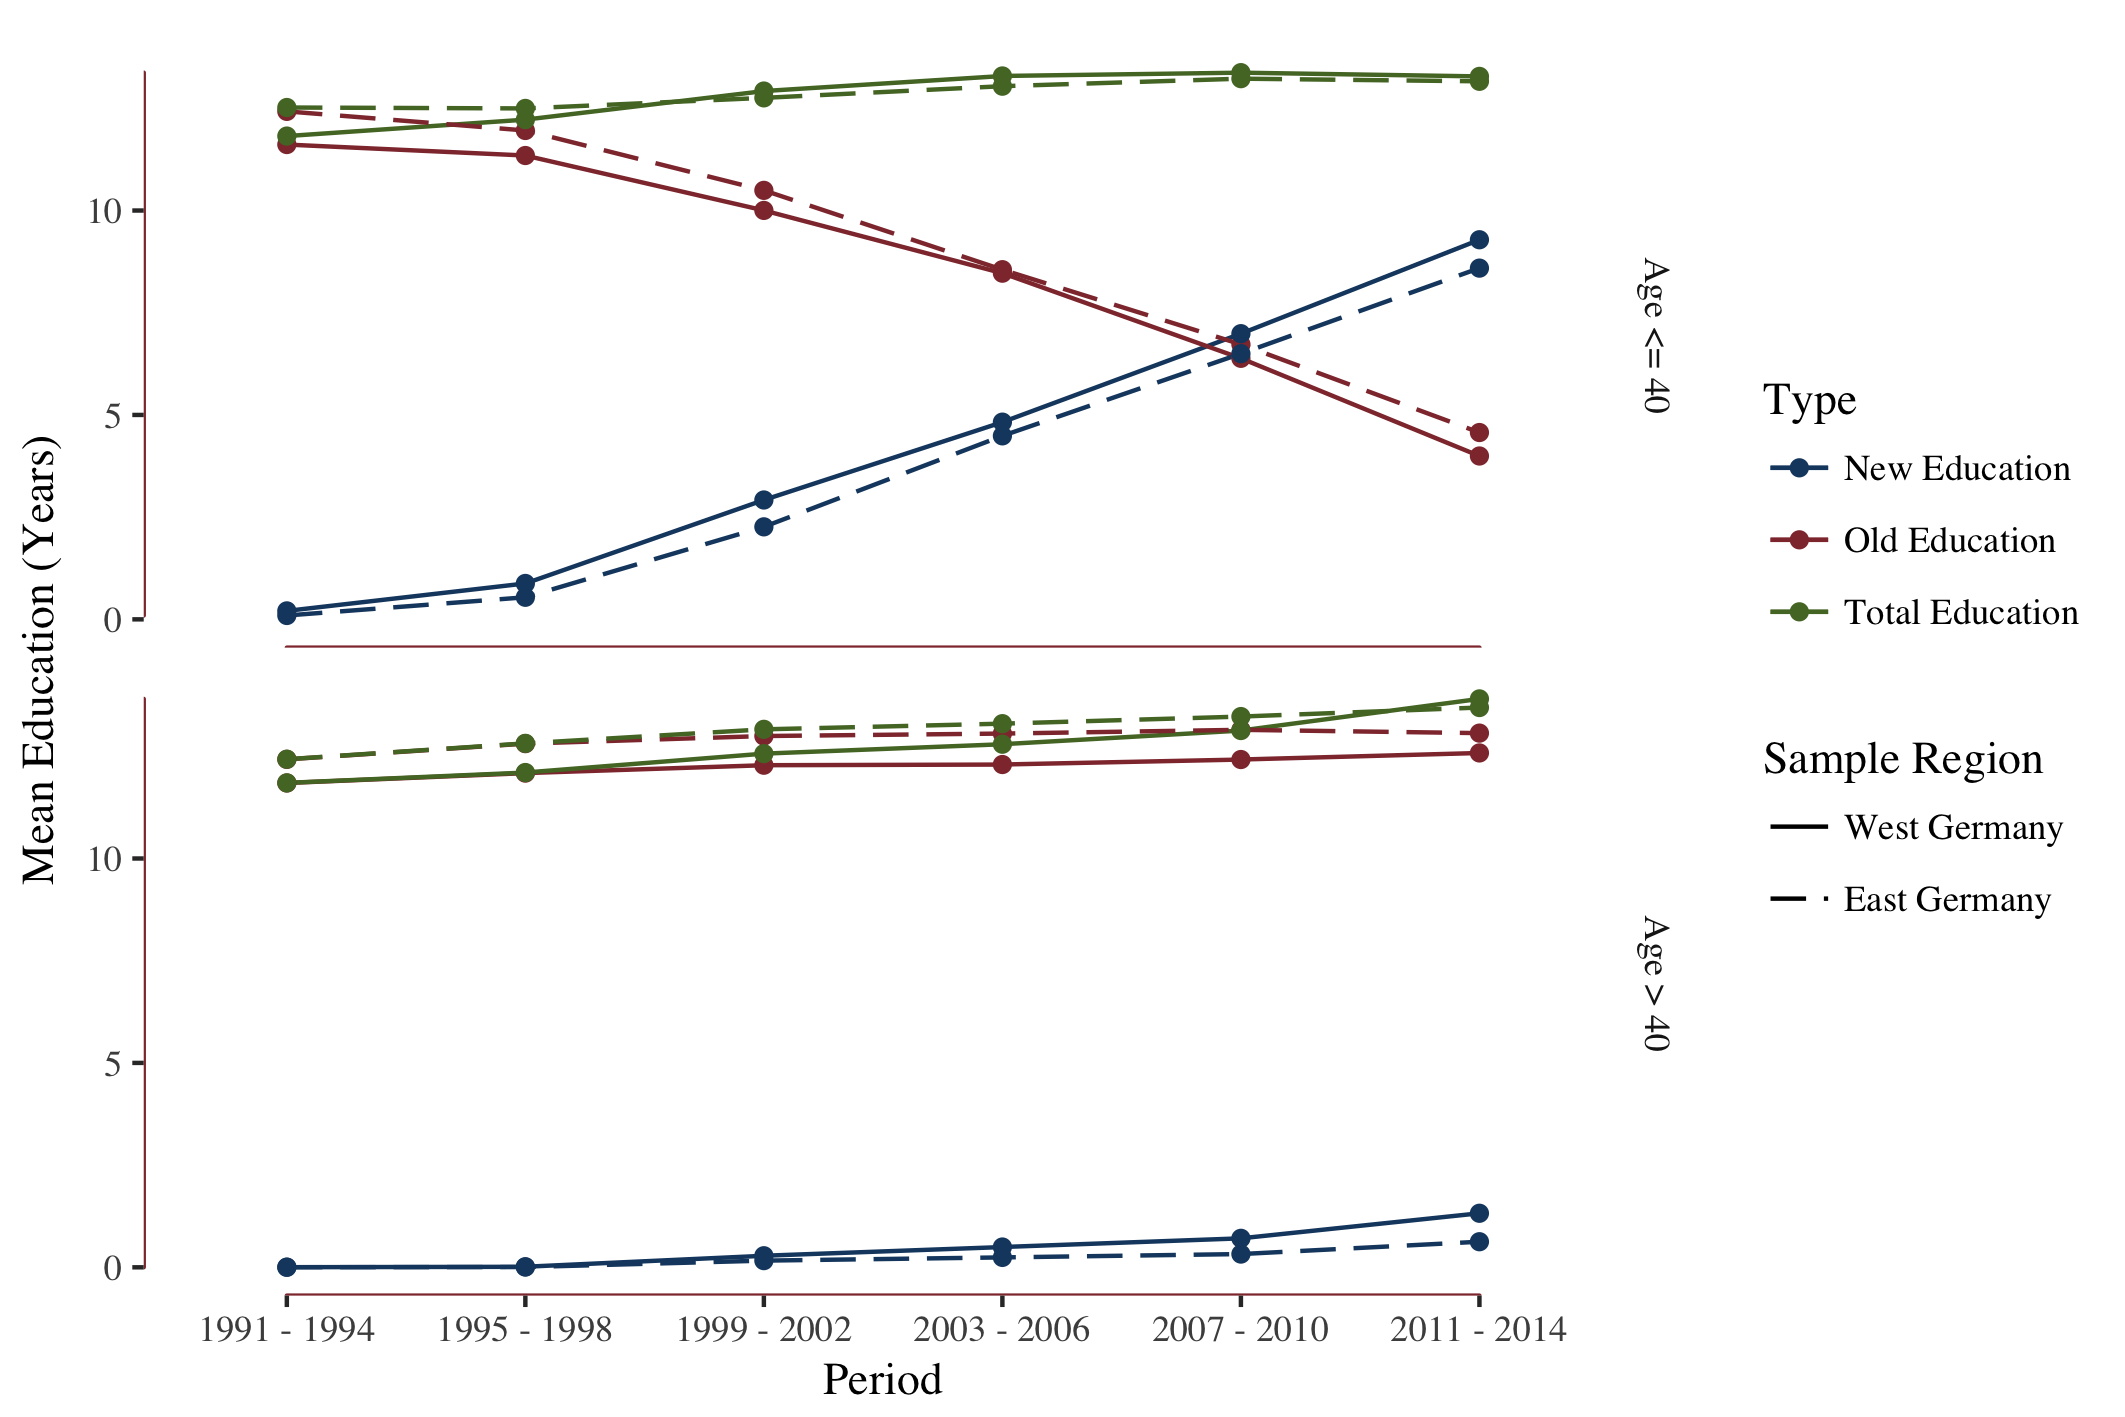
\includegraphics[width=\textwidth]{/Users/Christian/Statistik_Studium/EconProject/Code/Graphics/plotMeanEduByAgeGroup.png}
    \caption{Average Years of Education for two Age Groups}
    \label{fig:MeanEduByAgeGroup}
\end{figure}

\FloatBarrier
\section{Determinants of Wage}
\subsection{Model}
In this section the returns to Education and Experience will be analysed using two different kind of models:
\begin{equation}
	\begin{split}
	log(Wage) &= \beta_{1}TotalEdu + \beta_{2}TotalExp + \beta_{3} TotalExp^2\\
	&+\beta_{4}Tenure + \beta_{5}YearDummie + \beta_{6}Sex
	\end{split}
\end{equation}
\begin{equation} 
	\begin{split}
	log(Wage) &= \beta_{1a}OldEdu + \beta_{1b}NewEdu + \beta_{2a}OldExp \\
	&+ \beta_{2b}NewExp + \beta_{3a}OldExp^2 + \beta_{3b}NewExp^2\\
	&+\beta_{4}Tenure + \beta_{5}YearDummie + \beta_{6}Sex
	\end{split}
\end{equation}
These Models will be fitted using pooled OLS. All following results regarding Total Education and Experience are therefore based on the first model whereas all results regarding New and Old Experience or Education are based on the second one.
In the following I will give a short definition/explanation for each variable:

\begin{description}
	\item[TotalEdu] Total years of education gained both pre and post-reunification. This is the variable \textit{pgbilzt} from the \textit{SoepLong pgen} dataset. This variable is generated based on the type of degrees the individual obtained and is set to its minimum value 7 when no degree was obtained.
	\item[TotalExp] Total years of full time experience gained both pre- and post-reunification. This is the variable \textit{pexpft} from the \textit{SoepLong pgen} dataset.
	\item[Old Edu] Amount of Total Education gained before reunification. For most individuals this is set to the level of Total Education they had in 1990. For some younger individuals in later samples this is generated on the assumption that they started their education at age 6 and finished it consecutively.
	\item[Old Exp] Amount of Total Experience gained before reunification. For most individuals this is set to the level of Total Education they had in 1990. For some younger individuals in later samples this is set to zero if they have finished their education after reunification.
	\item[YearDummie] These are actually several dummie variables for each year in one period except the first, which is the reference year.
	\item[Tenure] Time spent with current employer (across different positions) in years. This is the variable \textit{pgerwzt} from the \textit{SoepLong pgen} dataset.
	\item[Sex] Dummie variable indicating whether an individual is female. 
	 
	
\end{description}

\subsection{Results by Region}
First we will fit seperate Models across region and time intervals to analyse relative changes in human capital in East and West Germany. 
To illustrate the changing returns to Education and Experience the predicted log wage gains from 0 to 5 years of experience and education are plotted in figures \ref{fig:DiffComparisonExp} and \ref{fig:DiffComparisonEdu}.  This is done, since because of the non-linearity of the Experience terms their effect would not be immediately obvious from the parameters and are not constant across the experience level. Looking at the returns to education one can observe several trends:
\begin{enumerate}
	\item Returns to Old Education from model 2 and returns to Total Education from model 1 are virtually identical across time and Sample Region.
	\item Rising Returns to all kinds of education across time with East German returns rising more quickly and overtaking West German levels in the early 2000s.
	\item Returns to New Education starting off at low levels but converging to those of Total and Old Education over time.	 
\end{enumerate}

\begin{figure}[!h]
    \centering
    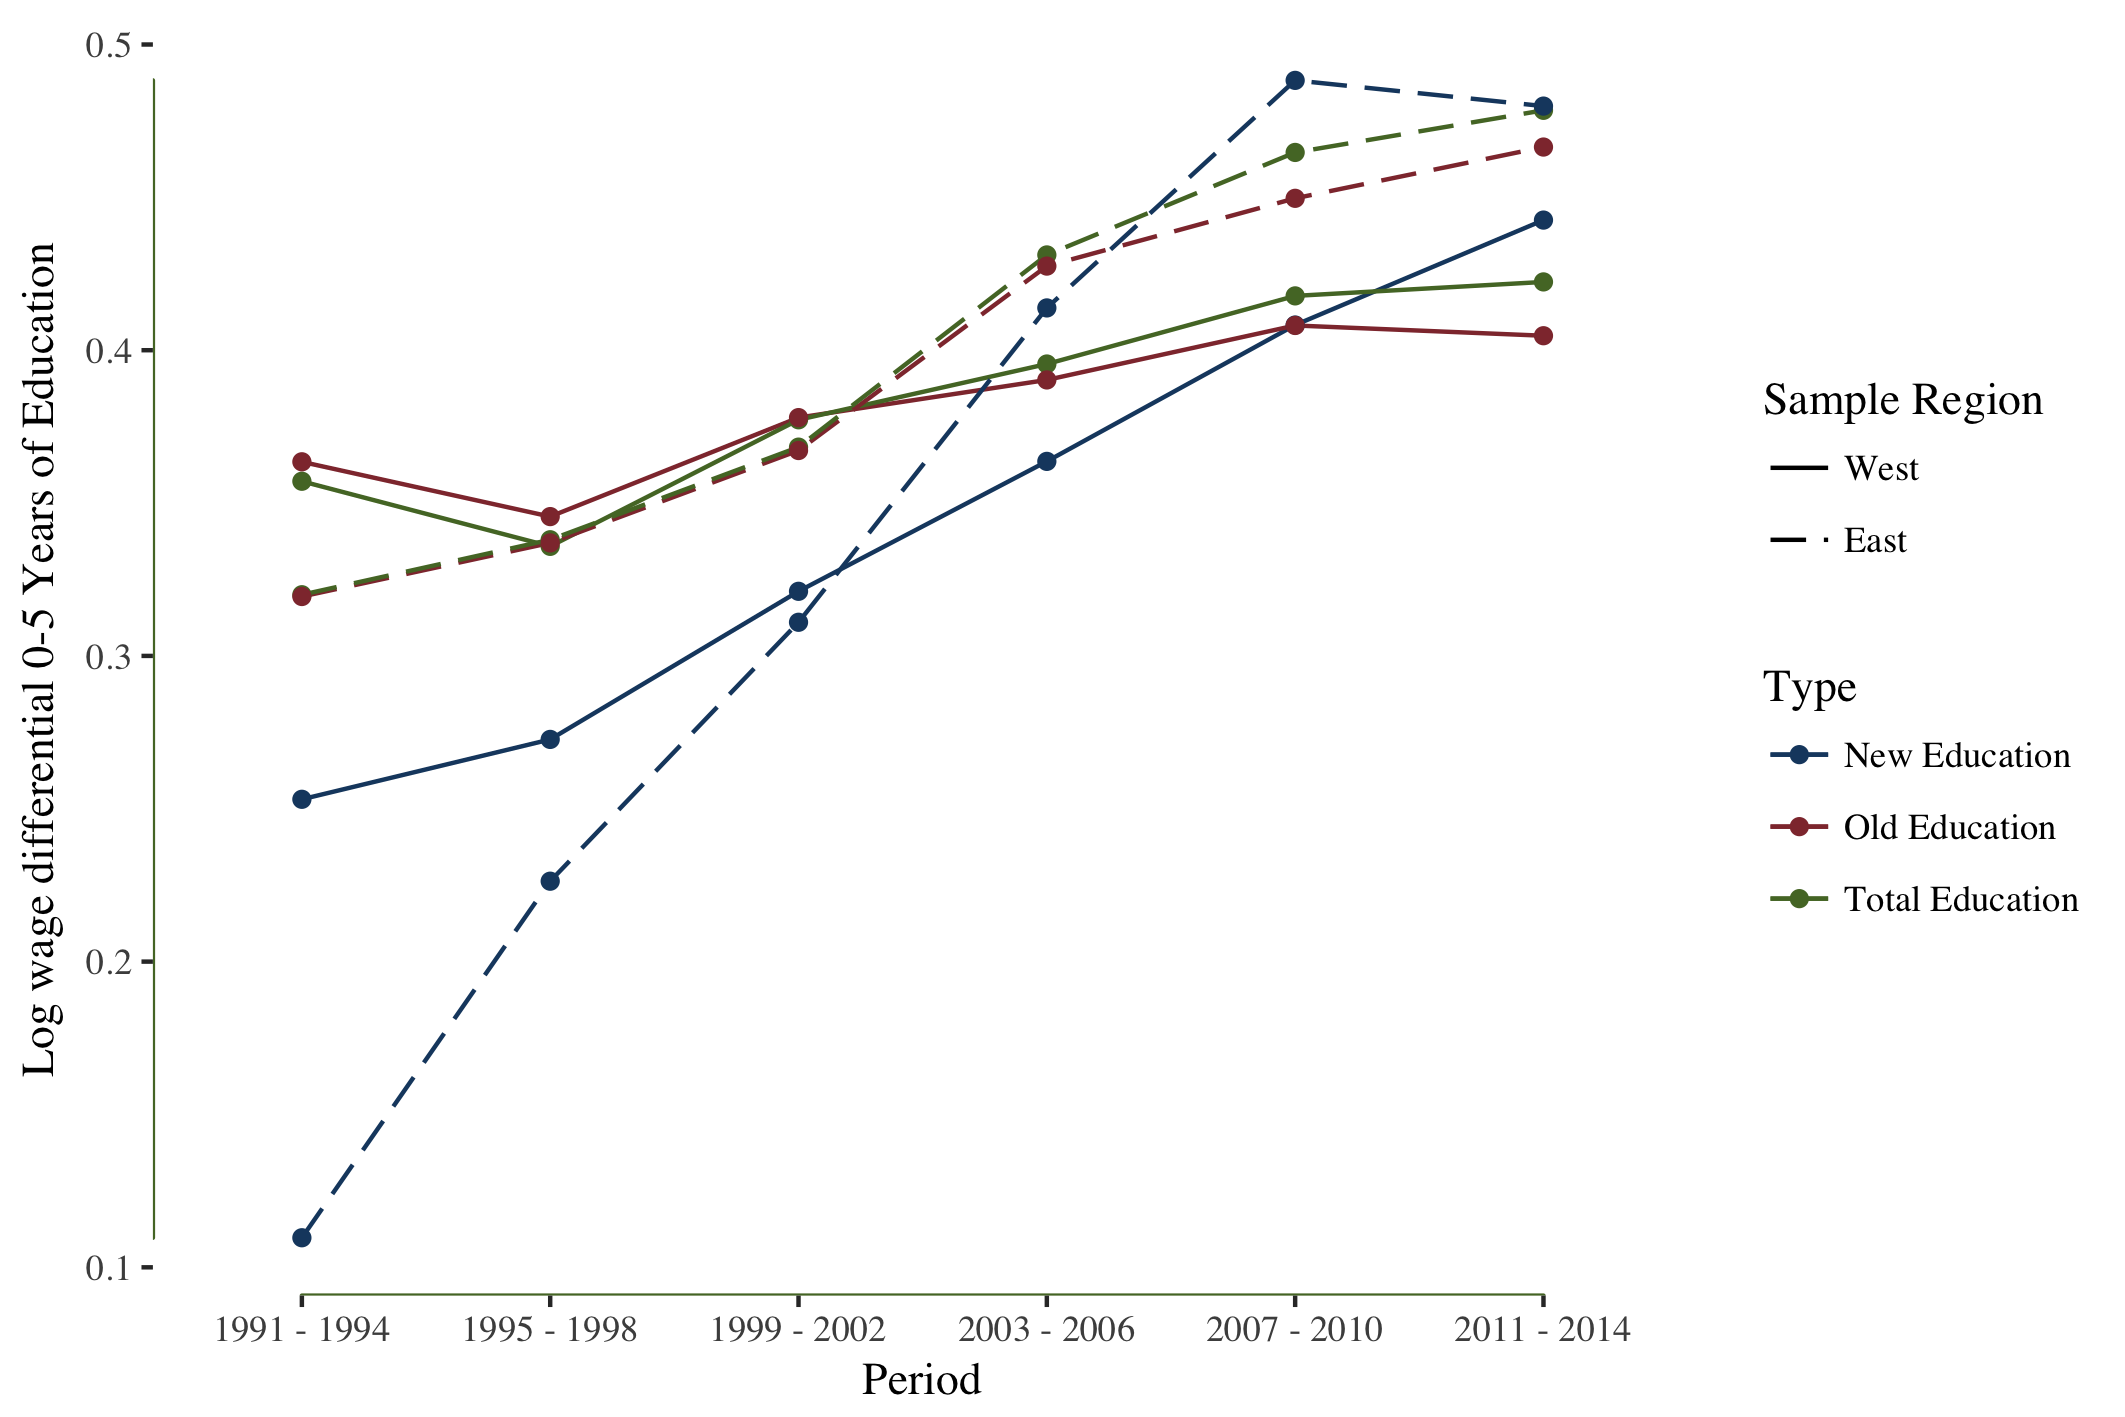
\includegraphics[width=\textwidth]{/Users/Christian/Statistik_Studium/EconProject/Code/Graphics/plotDiffComparisonEdu.png}
    \caption{Predicted Log Wage Difference 5-0 Years of Education}
    \label{fig:DiffComparisonEdu}
\end{figure}

Looking at the resulting returns to experience a very different picture emerges:
\begin{enumerate}
	\item Returns to New and Total Experience in West Germany constantly exceed those in the east
	\item Returns to Old Experience in East Germany are not significantly different from 0 in any period
	\item Returns to Old Experience in West Germany start of significantly different from 0 but converge to 0 over time.
	\item Returns to Total Experience lie somewhere between those of New and Old Experience across the timeframe
	\item Returns to New Experience converge to those of Total Experience
\end{enumerate}
\begin{figure}[!h]
    \centering
    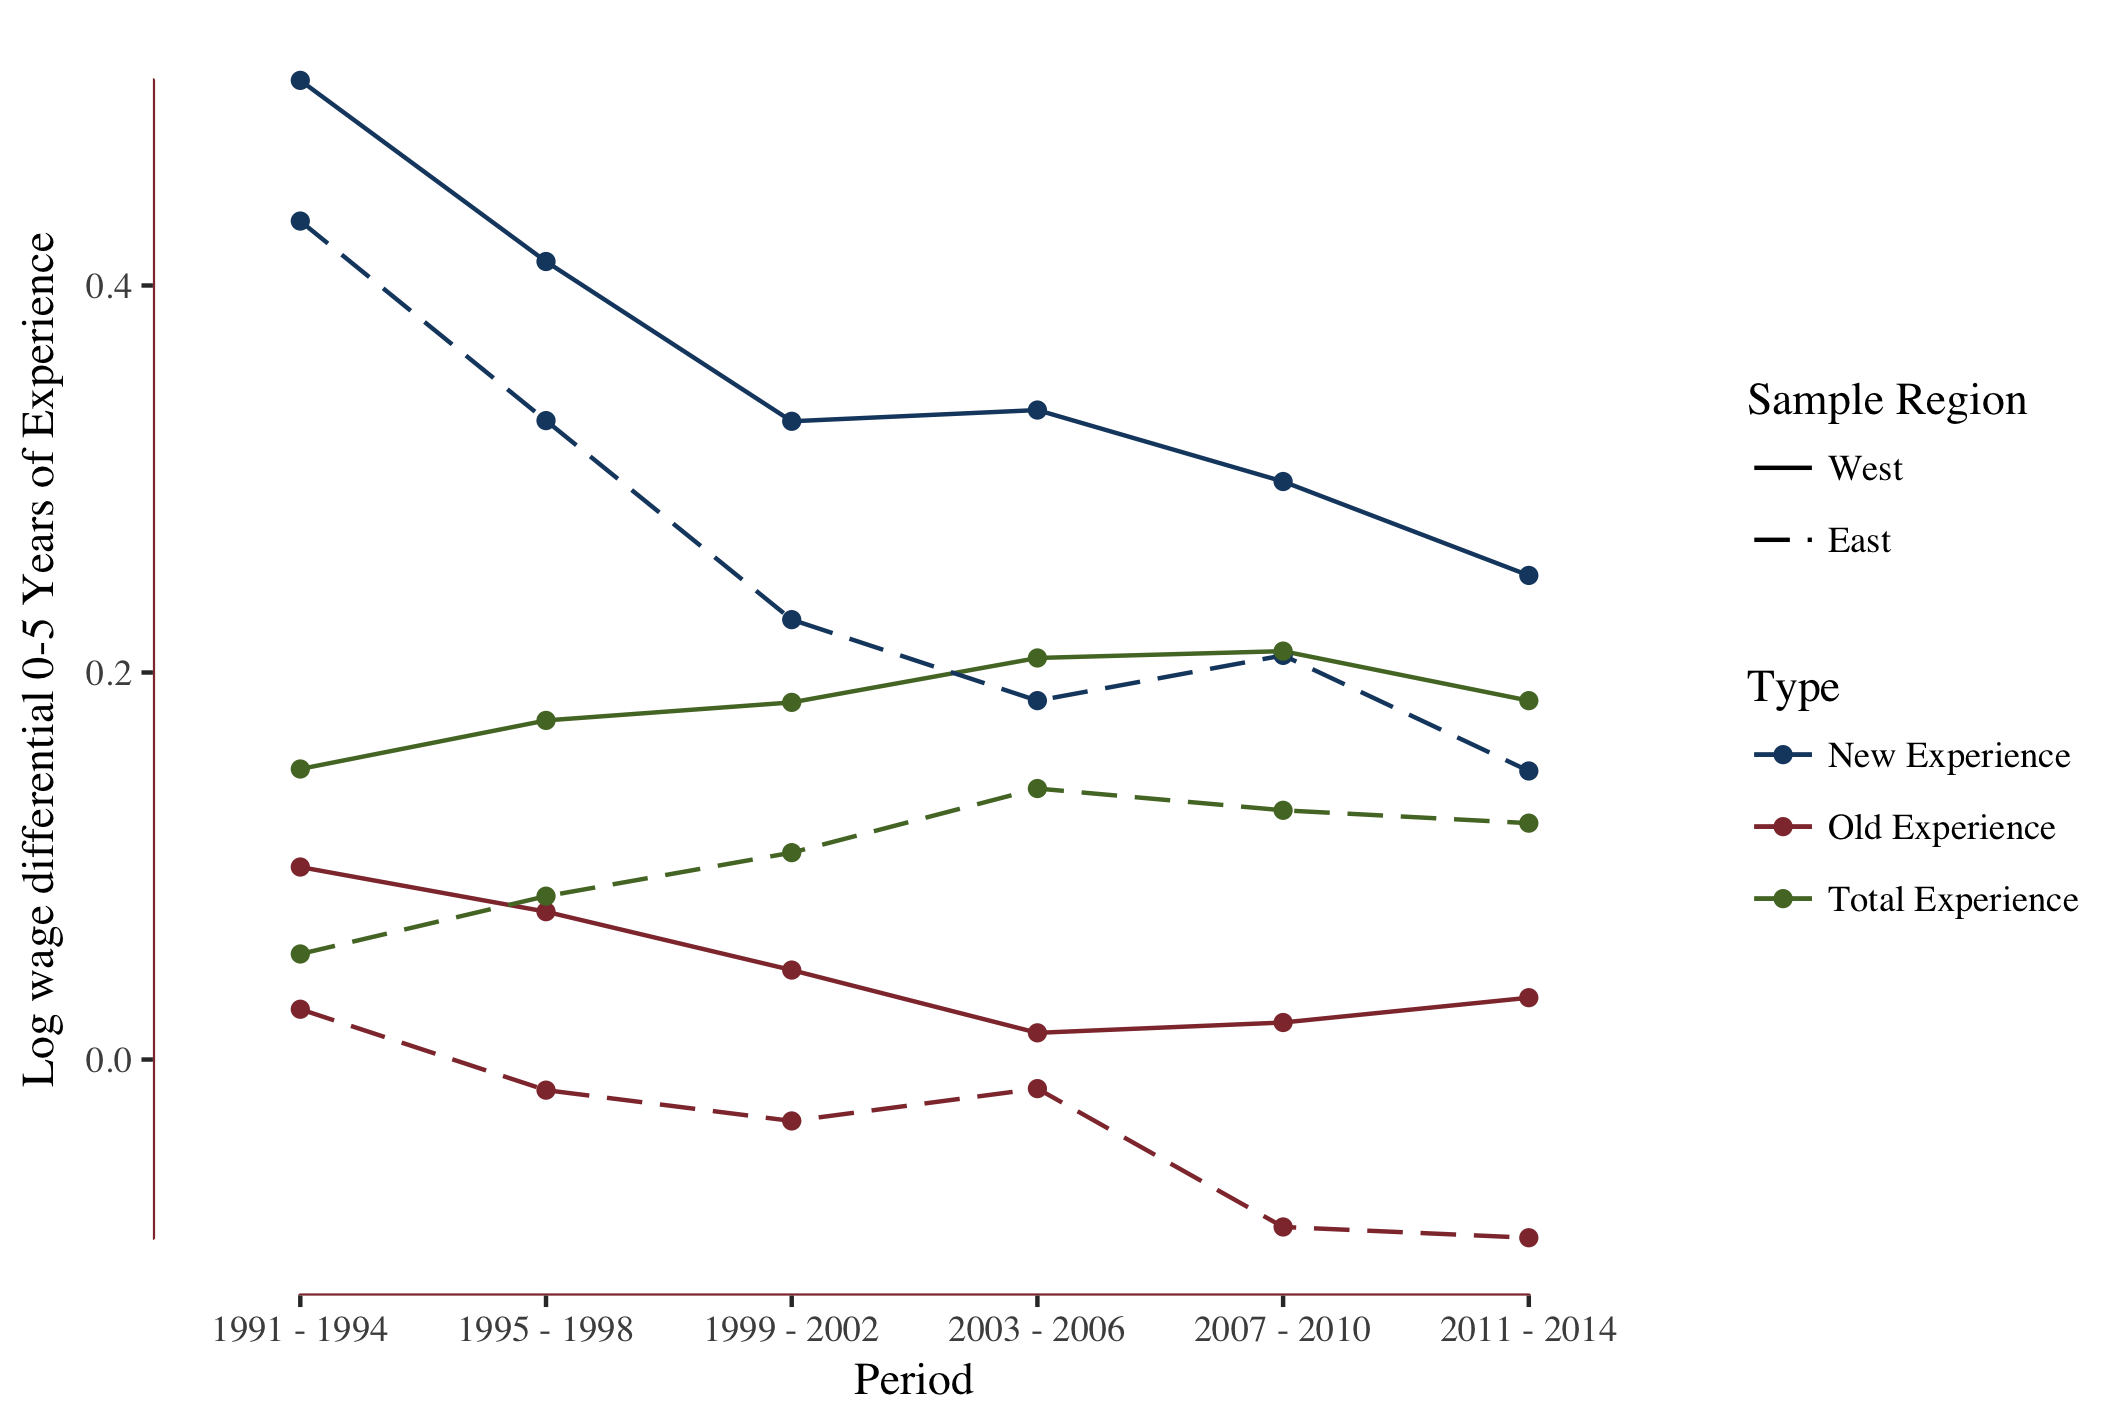
\includegraphics[width=\textwidth]{/Users/Christian/Statistik_Studium/EconProject/Code/Graphics/plotDiffComparisonExp.png}
    \caption{Predicted Log Wage Difference 5-0 Years of Experience}
    \label{fig:DiffComparisonExp}
\end{figure}


As seen in Figures \ref{fig:MeanEdu} and \ref{fig:MeanExp} however the sample populations in East and West Germany also differ according to the amount of Old- and New Experience as well as Education that they hold across time. Therefore the differences in the types of human capital that East and West Germans hold cannot be judged immediately when looking at wage returns for constant levels of education and experience (as we did with a constant value of 5 years above).  
Therefore in Figures \ref{fig:HumanCapitalExp} and \ref{fig:HumanCapitalEdu} the predicted returns are plotted when the constant level of five is replaced with year and sample region specific averages from Figures \ref{fig:MeanEdu} and \ref{fig:MeanExp}. 

From figure \ref{fig:HumanCapitalExp} one can again take away several observations regarding Human Capital in Experience for East and West Germany:

\begin{enumerate}
	\item The estimated human capital in Old Experience for East Germans is constantly almost zero and even negative starting from the second period.
	\item The West German Population starts off with a significant share of human capital in Old Experience that converges towards zero throughout the 1990's.
	\item The human capital in new experience rises throughout the time frame with West German levels exceeding East German ones by a relatively constant margin. 
\end{enumerate}

Regarding the human capital stored in education (Figure \ref{fig:HumanCapitalEdu}) however we conclude the following:

\begin{enumerate}
	\item A rising share of human capital in education is stored in New Education although this process happens considerably faster in West than in East Germany. This is mainly due to a similar behaviour in Mean Levels of Education observed in Figure \ref{fig:MeanEdu}.
	\item While the amount of Human Capital in Old Education is relatively constant in East Germany it falls in the West German sample.
	\item Overall Human Capital in Education is relatively similar between sample regions, with East German levels rising above West German ones towards the end of the time frame.
\end{enumerate}



\begin{figure}[!h]
    \centering
    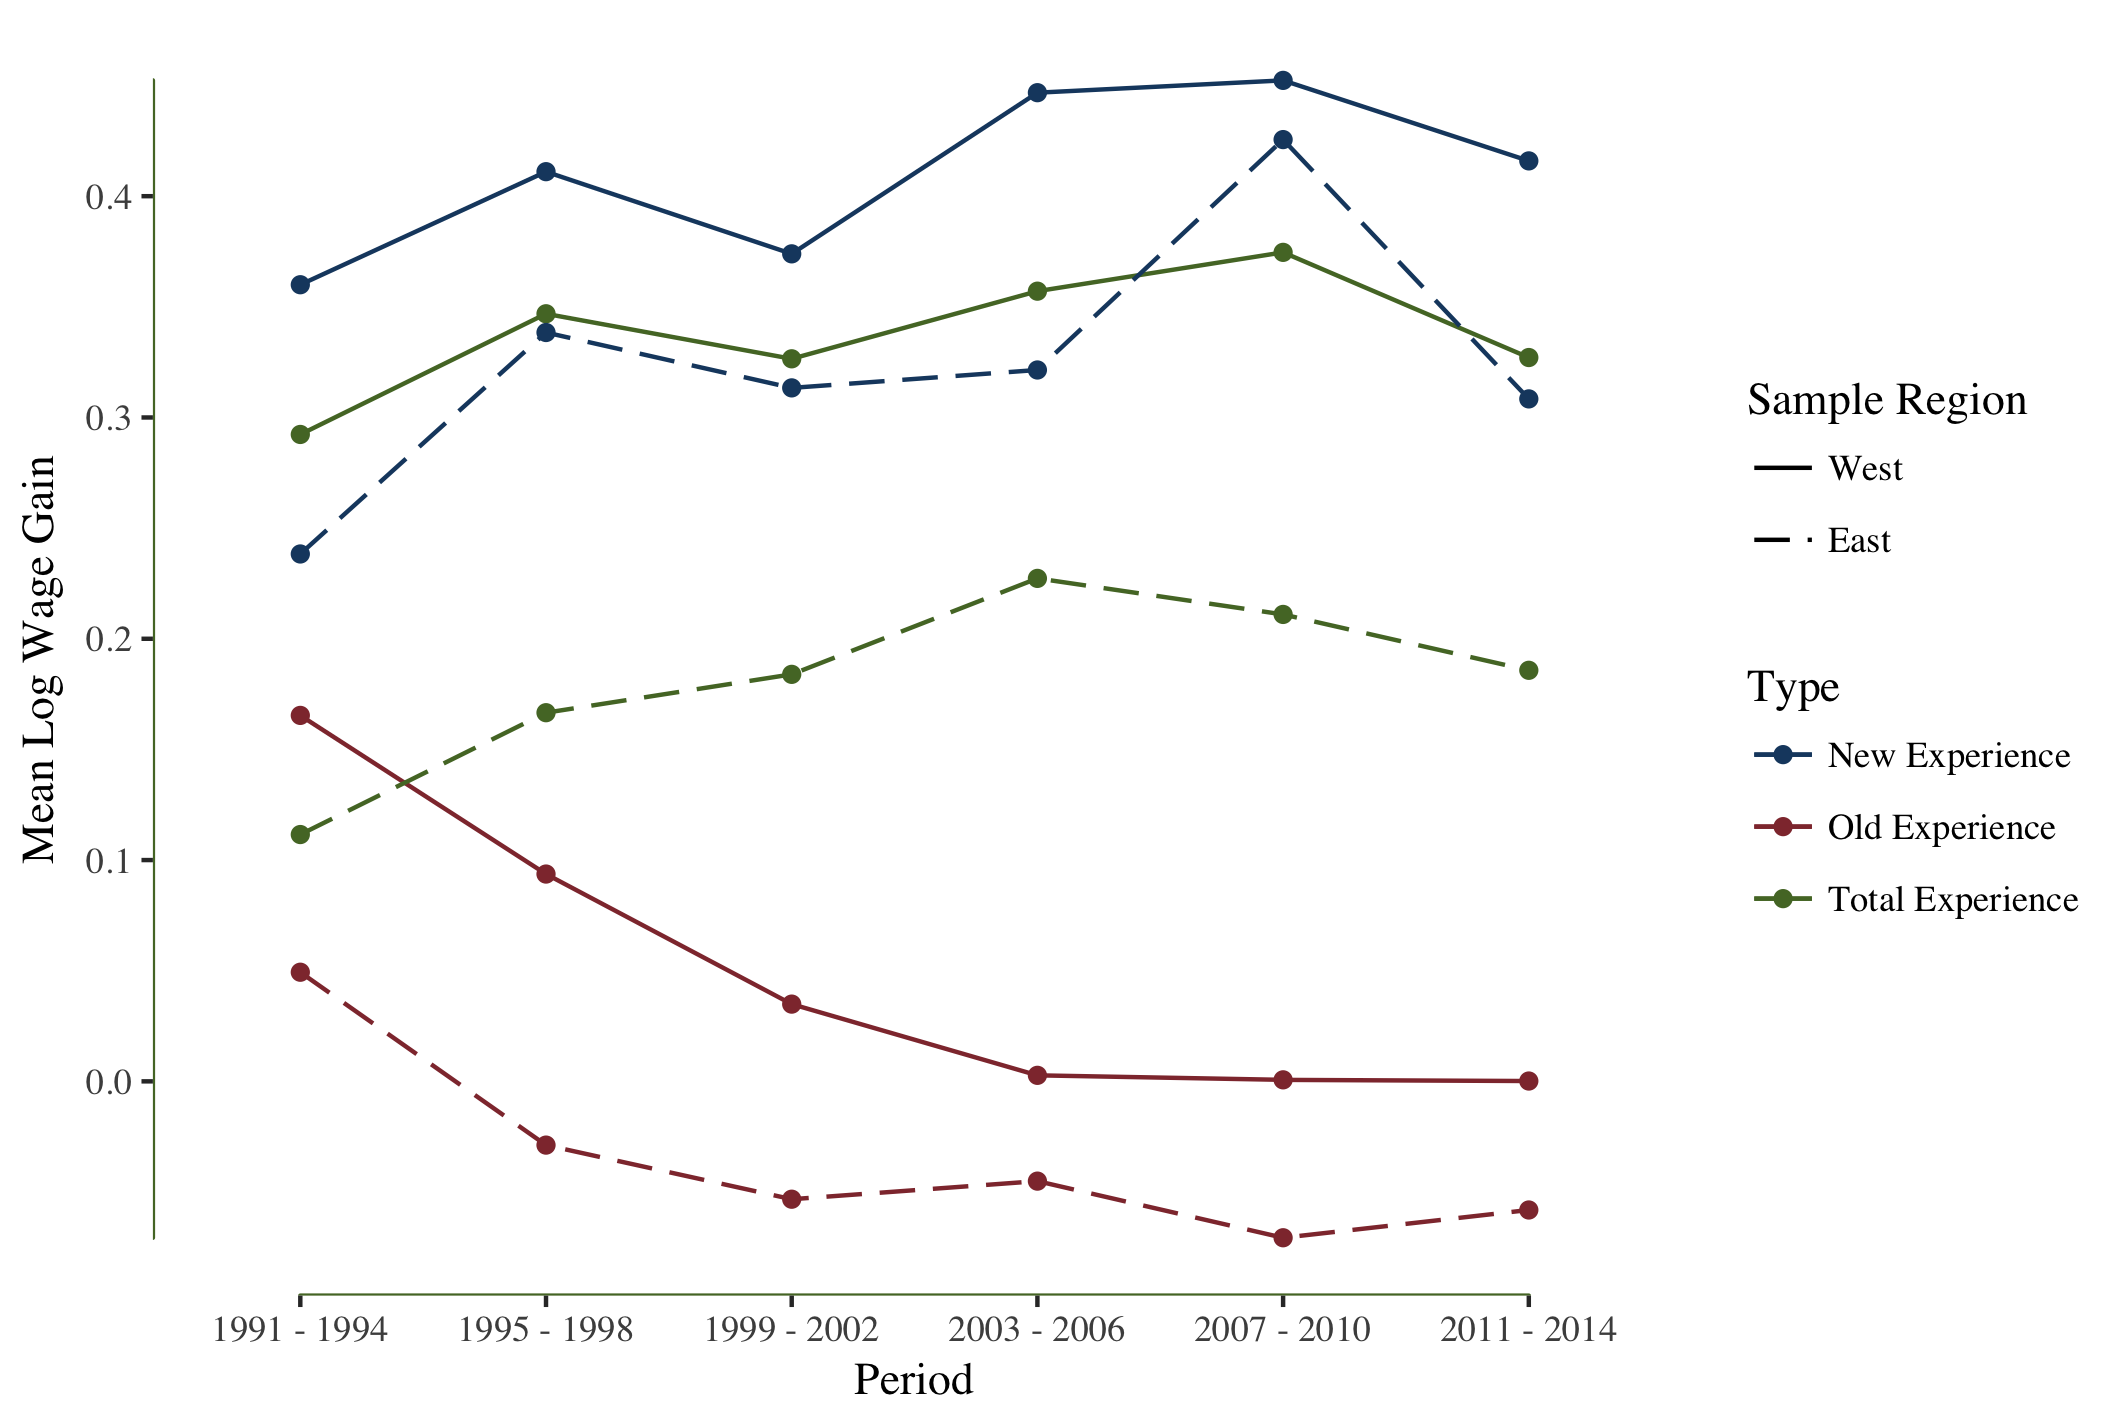
\includegraphics[width=\textwidth]{/Users/Christian/Statistik_Studium/EconProject/Code/Graphics/plotHumanCapitalExp.png}
    \caption{Predicted Log Wage Difference for year and sample region specific Mean Years of Experience}
    \label{fig:HumanCapitalExp}
\end{figure}

\begin{figure}[!h]
    \centering
    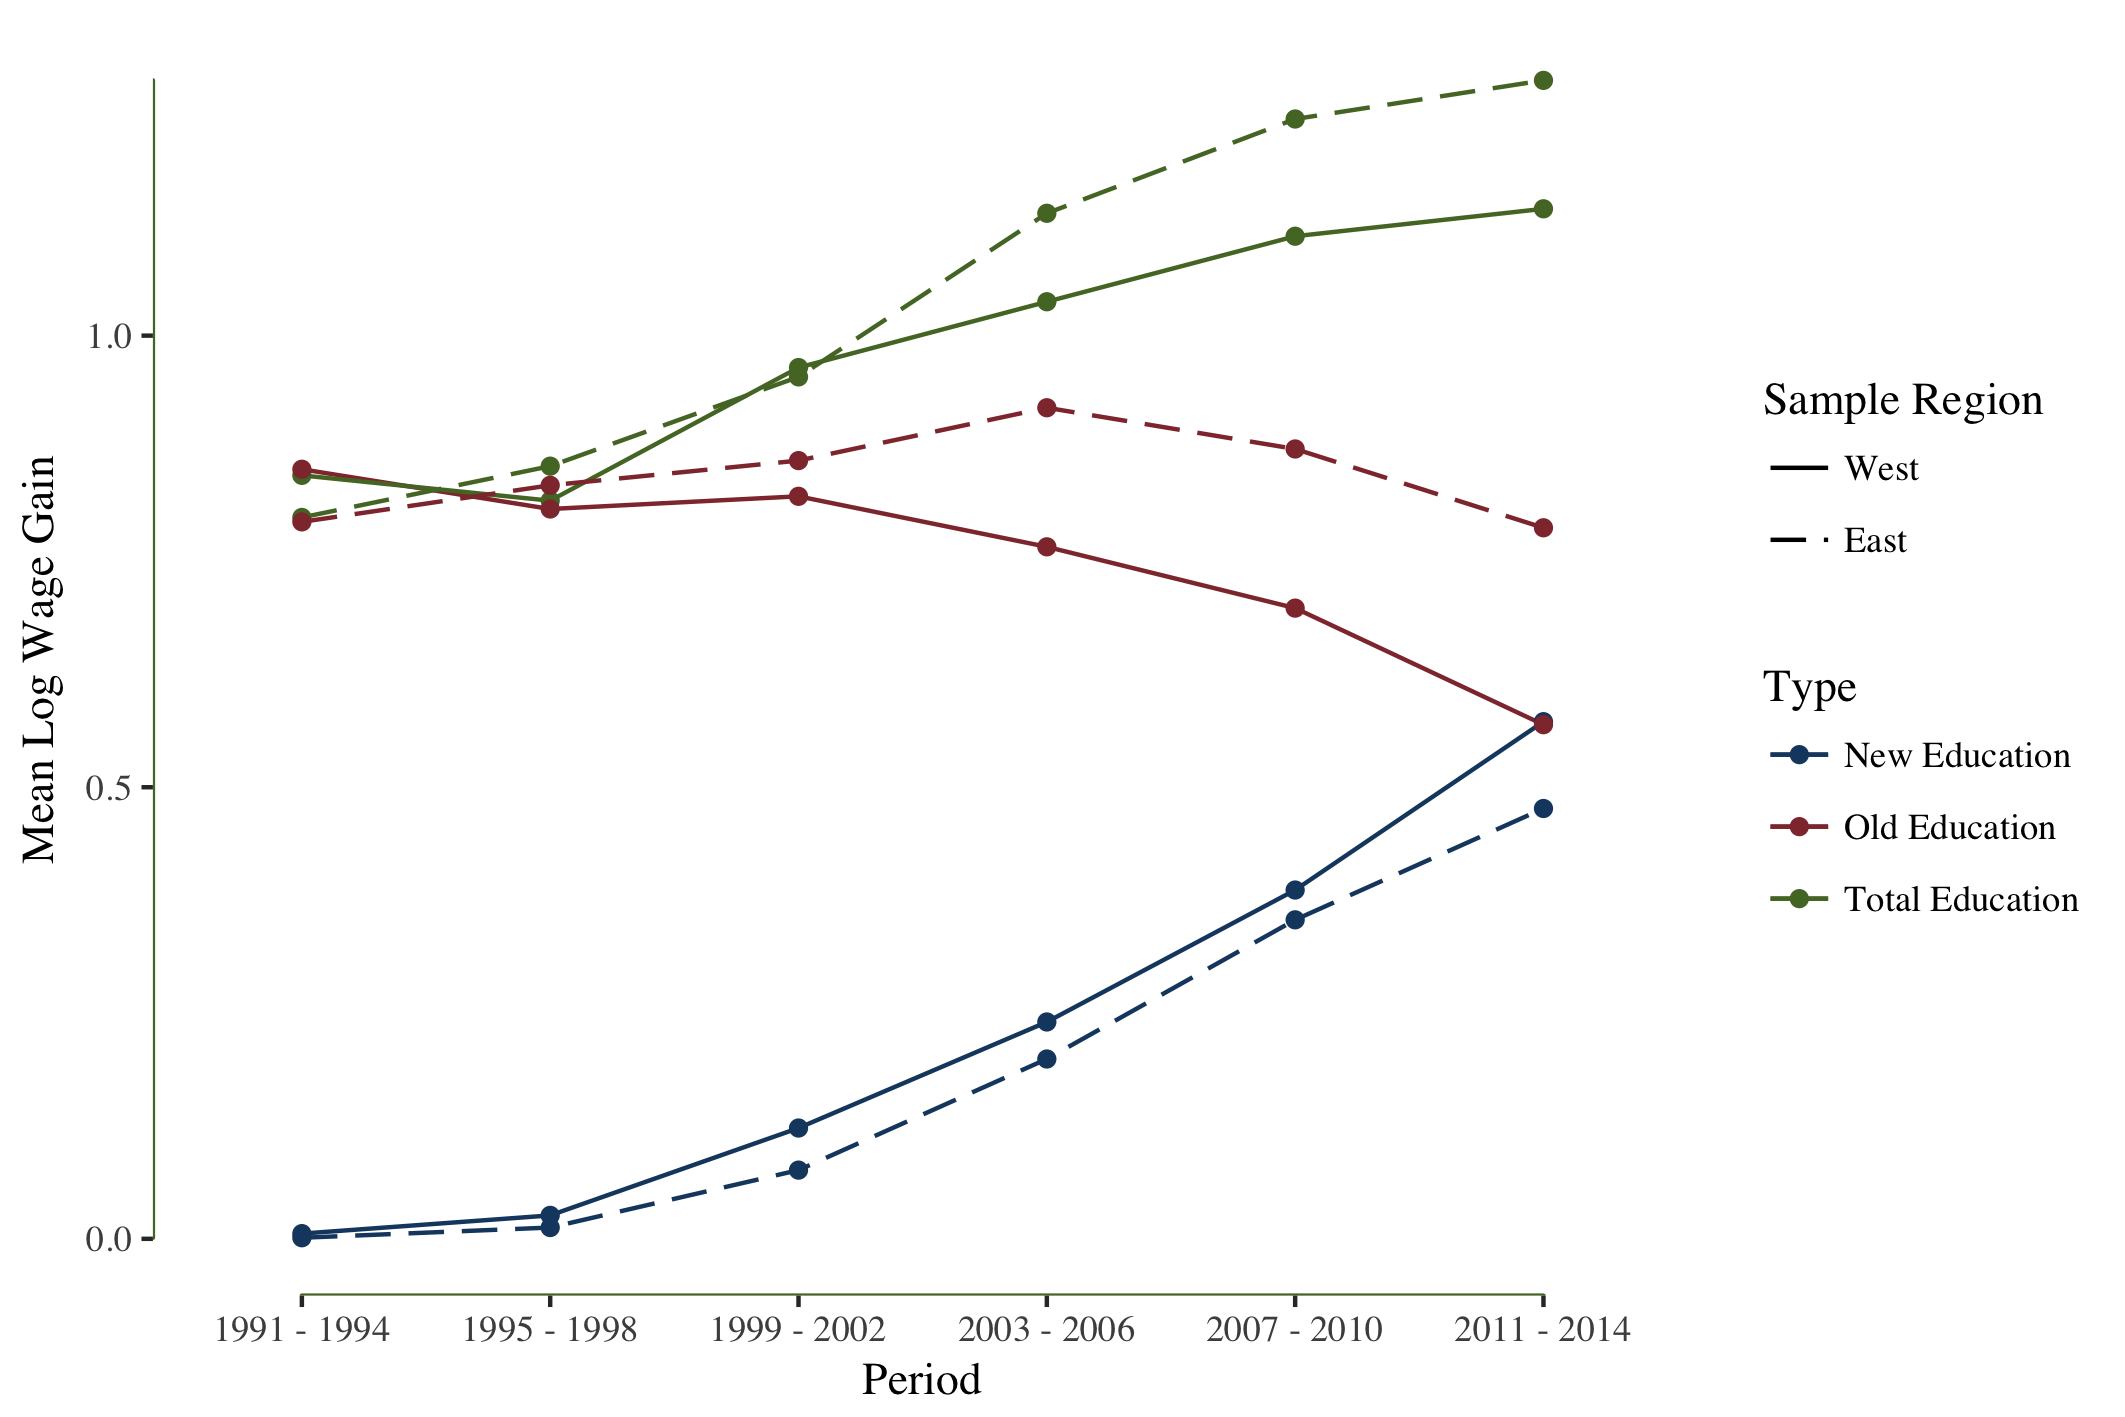
\includegraphics[width=\textwidth]{/Users/Christian/Statistik_Studium/EconProject/Code/Graphics/plotHumanCapitalEdu.png}
    \caption{Predicted Log Wage Difference for year and sample region specific Mean Years of Education}
    \label{fig:HumanCapitalEdu}
\end{figure}

\FloatBarrier
\subsection{Results by Region and Age Group}
In this section we will analyse the returns when the data is not just separated by Year and Region but also by age group. In this context we separate the populations in Young and Old individuals, where the separation is done at the age of 40 years. Figures \ref{fig:DiffComparisonExpByAgeGroup} and \ref{fig:HumanCapitalExpByAgeGroup} display equivalent Graphs to those in Figures  \ref{fig:DiffComparisonExp} and \ref{fig:HumanCapitalExp} for each age group.

From figure \ref{fig:DiffComparisonExpByAgeGroup} we observe the following regarding the returns to experience:

\begin{enumerate}
	\item For young individuals from both regions there is a slight decrease in the returns to new education which are almost identical to the returns of total experience from the late nineties onwards.
	\item Young West Germans enjoy higher returns to education than their eastern peers, a difference that slowly decreases but is still visible in the last time period.
	\item Old Germans in both regions exhibit high returns to new education immediately after reunification which quickly converge to zero and even enter negative territory in the early 2000s.
\end{enumerate}

\begin{figure}[!h]
    \centering
    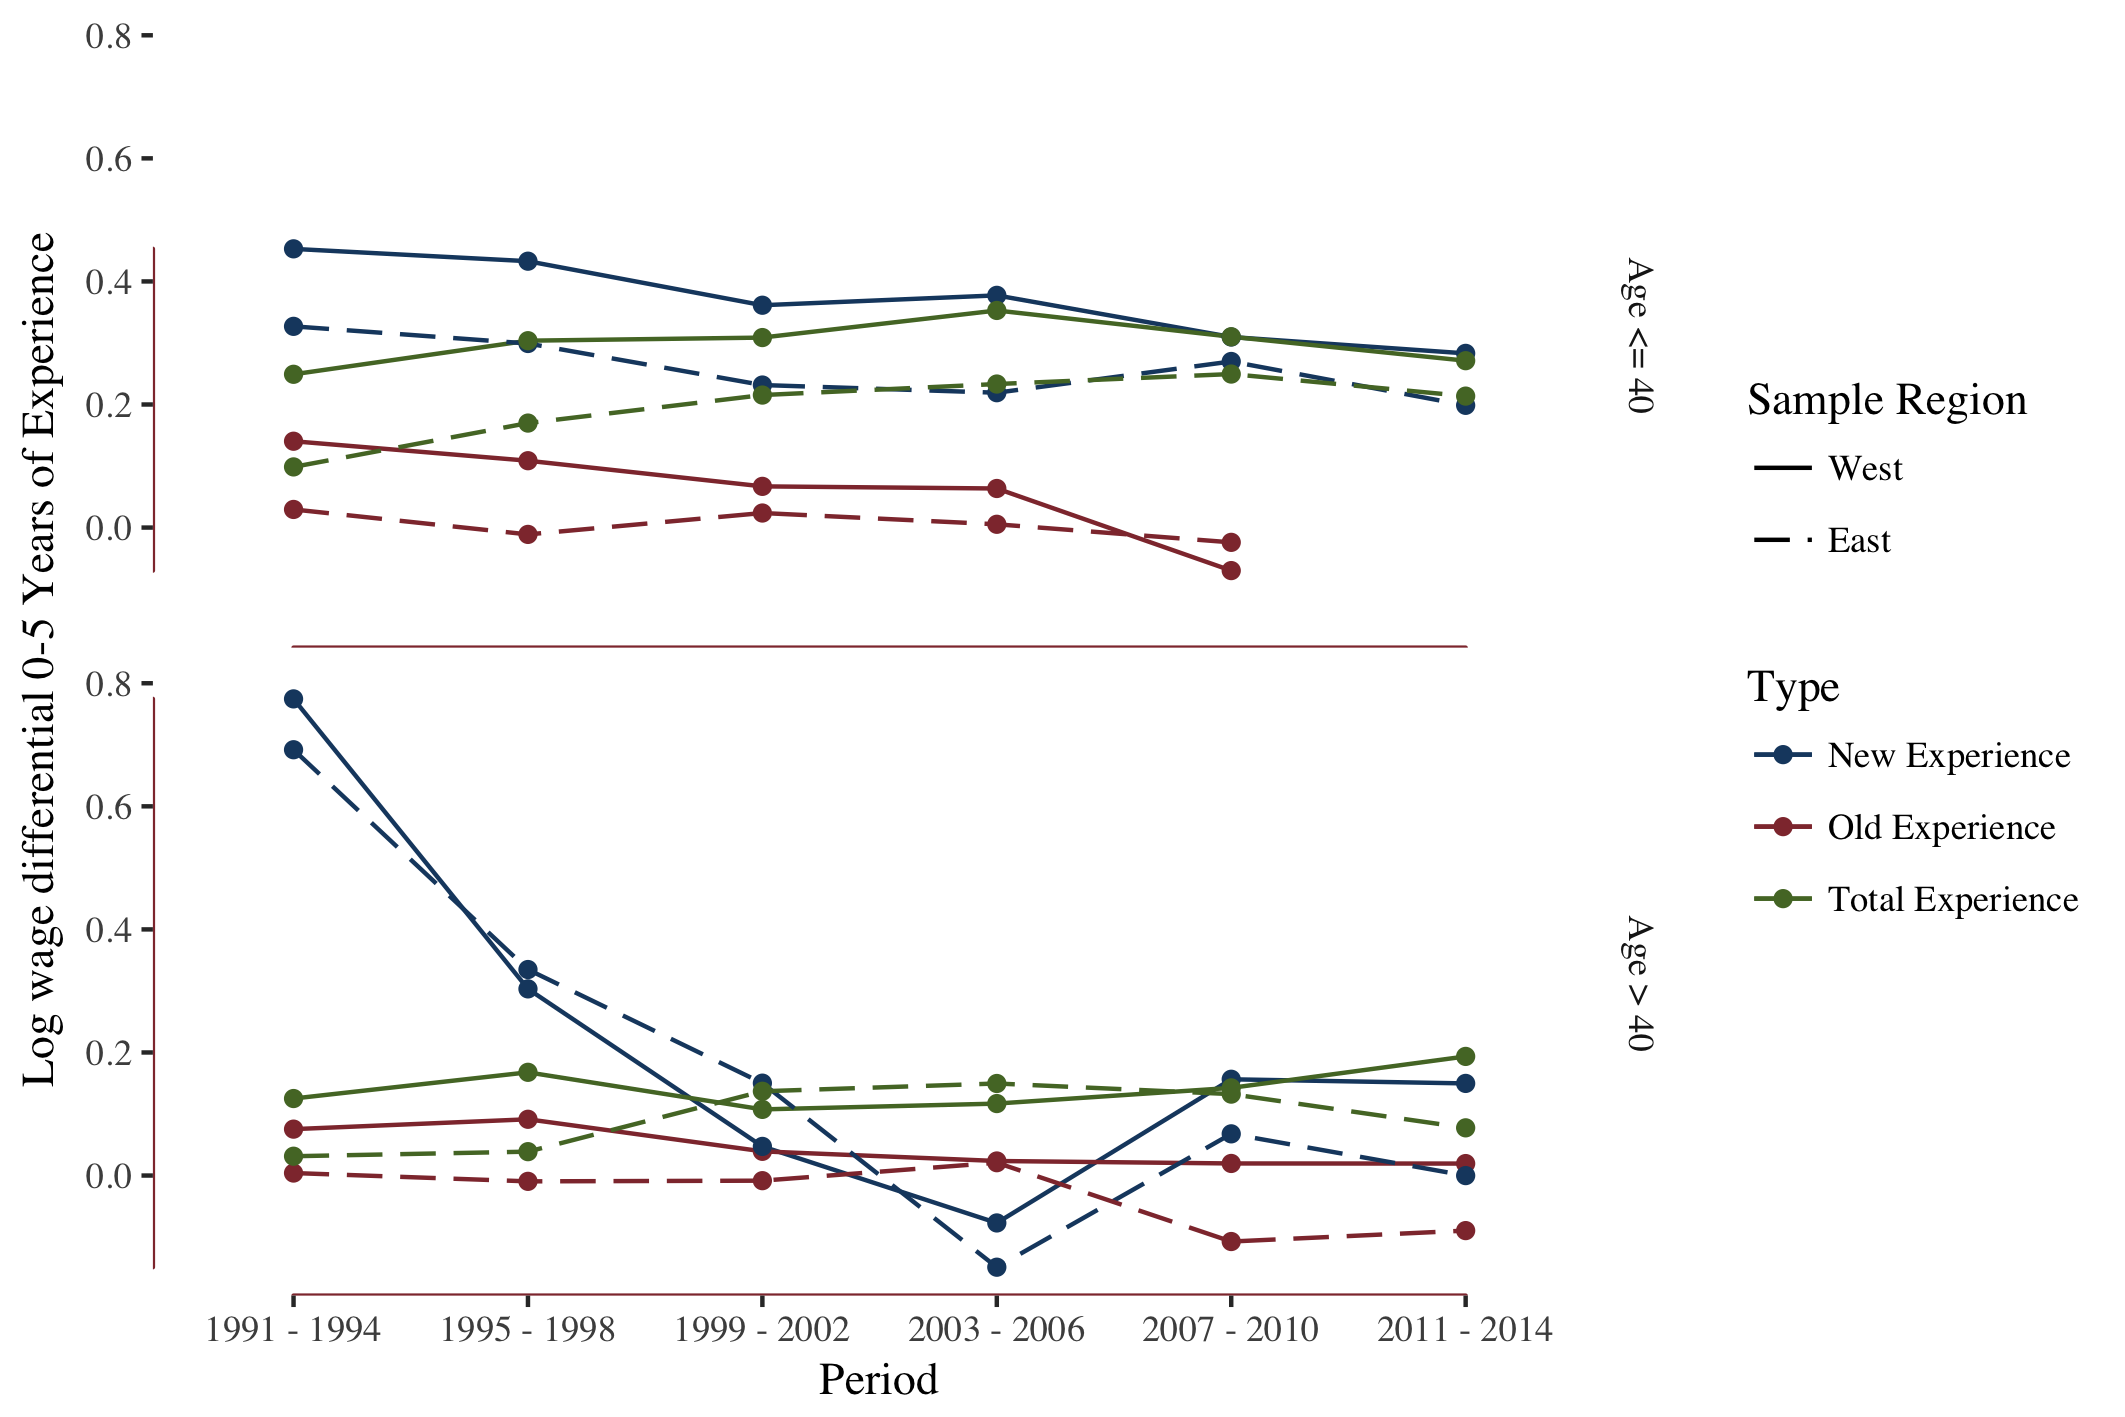
\includegraphics[width=\textwidth]{/Users/Christian/Statistik_Studium/EconProject/Code/Graphics/plotDiffComparisonExpByAgeGroup.png}
    \caption{Predicted Log Wage Difference 5-0 Years of Experience}
    \label{fig:DiffComparisonExpByAgeGroup}
\end{figure}

Regarding human capital in experience we observe the following from figure \ref{fig:HumanCapitalExpByAgeGroup}:

\begin{enumerate}
	\item For young individuals the estimated human capital in new and total experience are virtually identical throughout the time frame.
	\item The human capital in new and total experience is relatively constant for young individuals with western levels exceeding eastern ones throughout the time frame.
	\item The estimated human capital of old individuals shows very unstable behaviour and no clear pattern.

\end{enumerate}


\begin{figure}[!h]
    \centering
    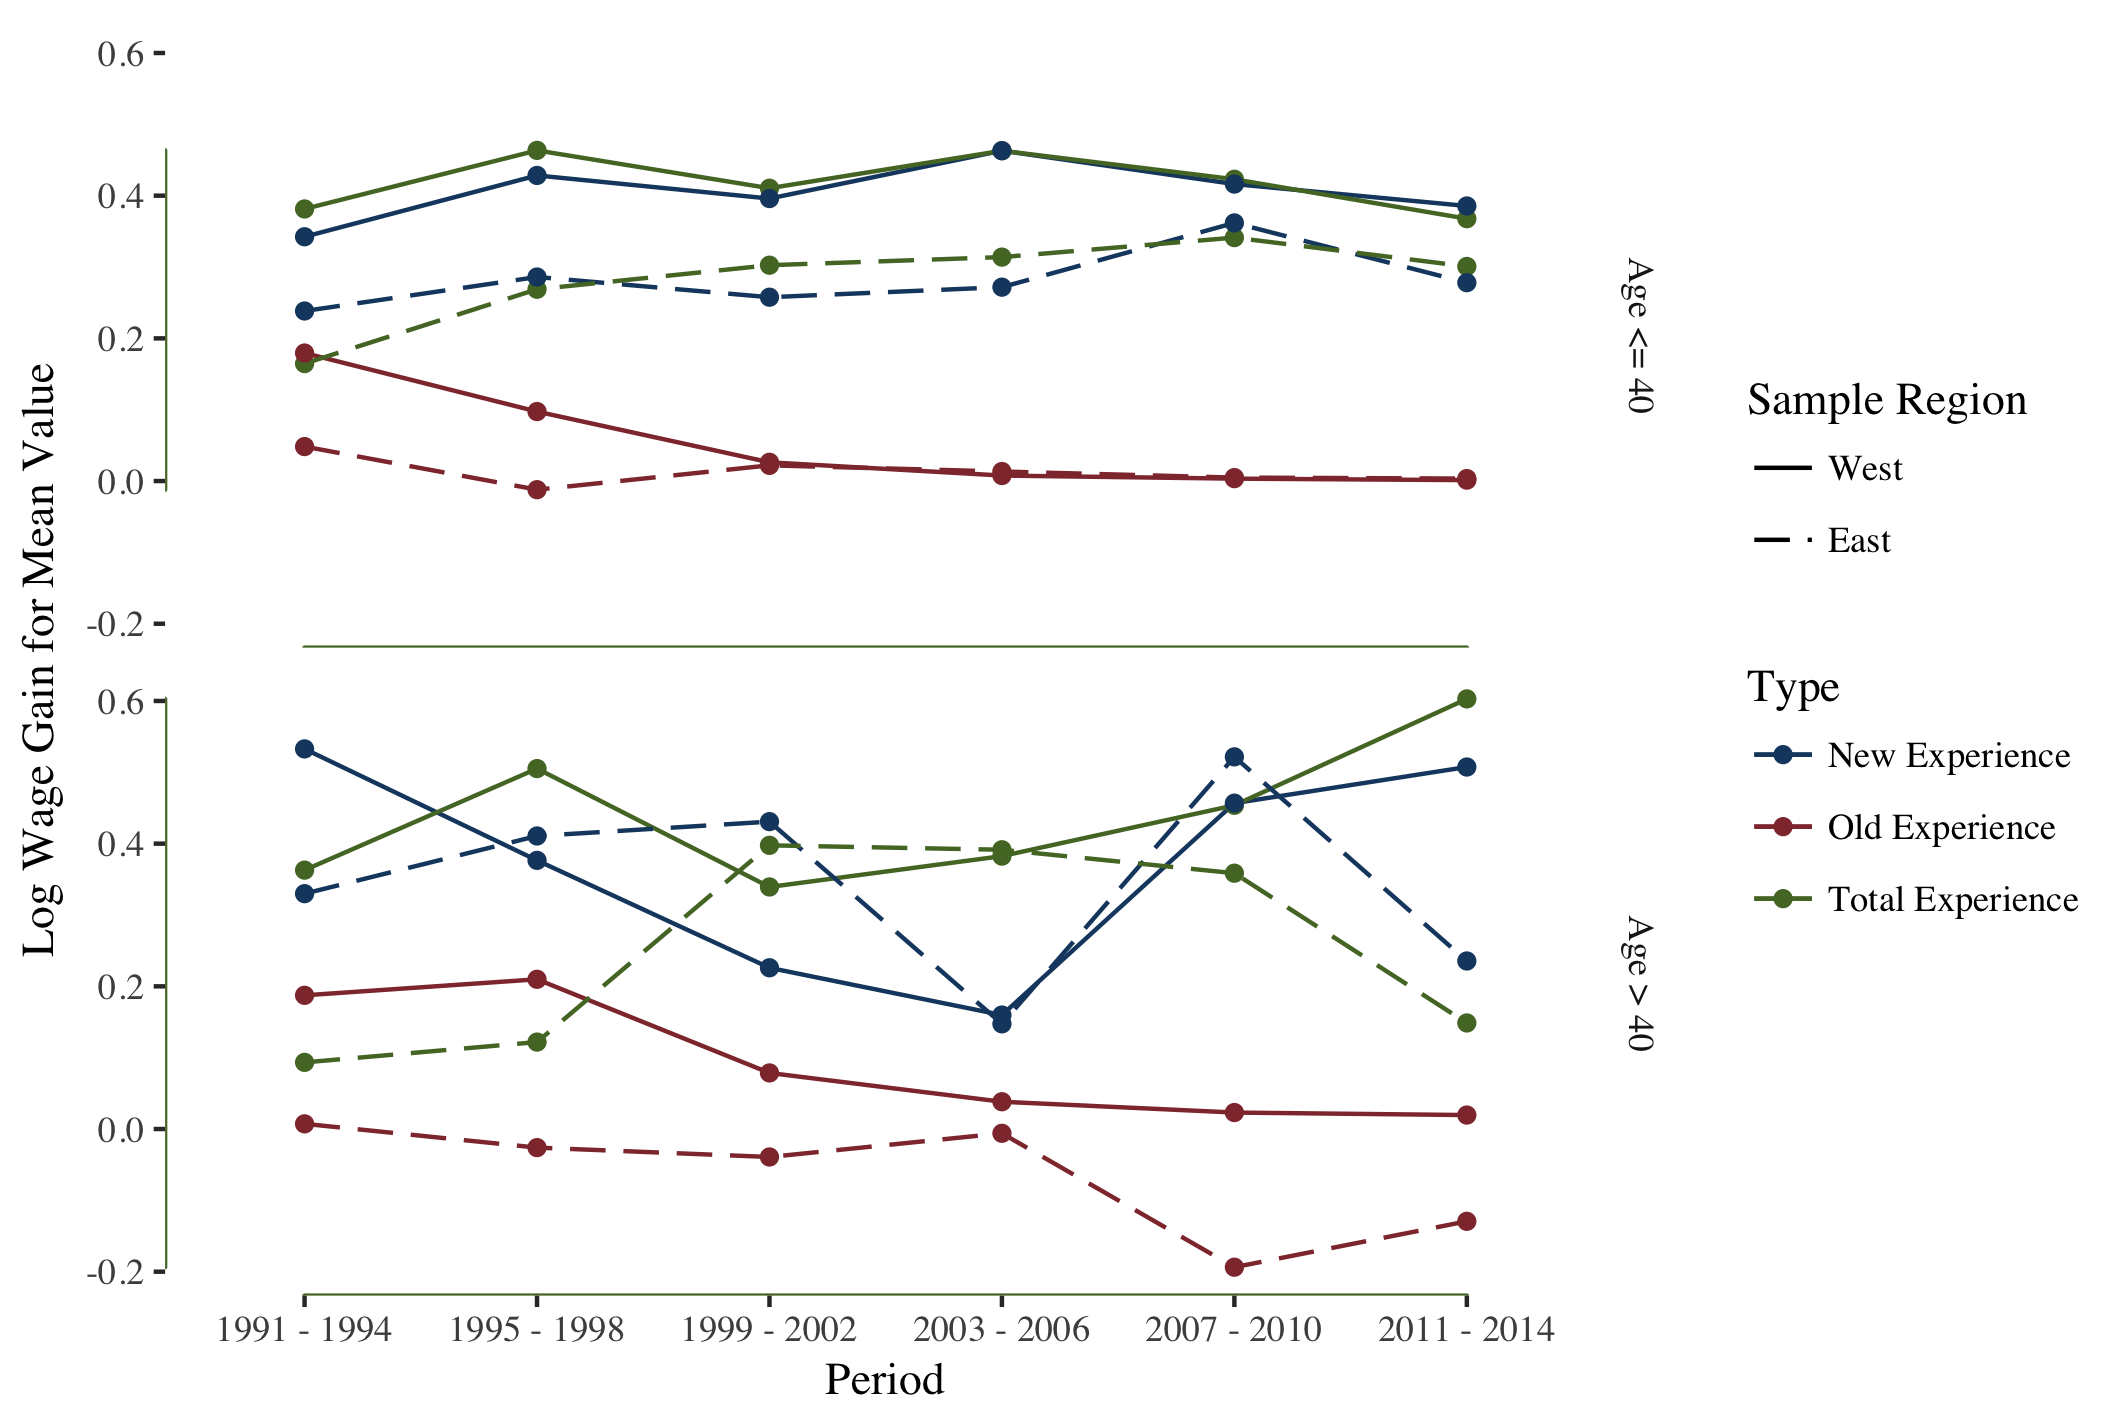
\includegraphics[width=\textwidth]{/Users/Christian/Statistik_Studium/EconProject/Code/Graphics/plotHumanCapitalExpByAgeGroup.png}
    \caption{Predicted Log Wage Difference for Mean Years of Experience separated by Age Group}
    \label{fig:HumanCapitalExpByAgeGroup}
\end{figure}

\FloatBarrier
\subsection{Results by Region and Skill Group}
In this section the additional criteria of separation is the Skill Group of the Individual, which is defined by the highest degree (No Vocational, Vocational, College Degree).

By looking at the results for returns to experience  we obtain the following observations:

\begin{enumerate}
	\item Returns to Old Experience are low across Skill Groups
	\item Regional differences in returns to all types of experience are almost zero for workers with a vocational degree throughout the timeframe
	\item Regional differences in the returns to experience are highest in the group of college graduates.
\end{enumerate}

From Figure \ref{fig:HumanCapitalExpBySkillGroup} we observe the following regarding Human Capital.

\begin{enumerate}
	\item Human Capital in New and Total Experience converge towards similar levels for both the College and No Vocational Degree groups. This process seems to occur more quickly though for the No Vocational Degree group.
	\item Regional differences in Human Capital start out at smaller levels for the Vocational Degree group but stay relatively constant throughout the time frame.

\end{enumerate}

\begin{figure}[!h]
    \centering
    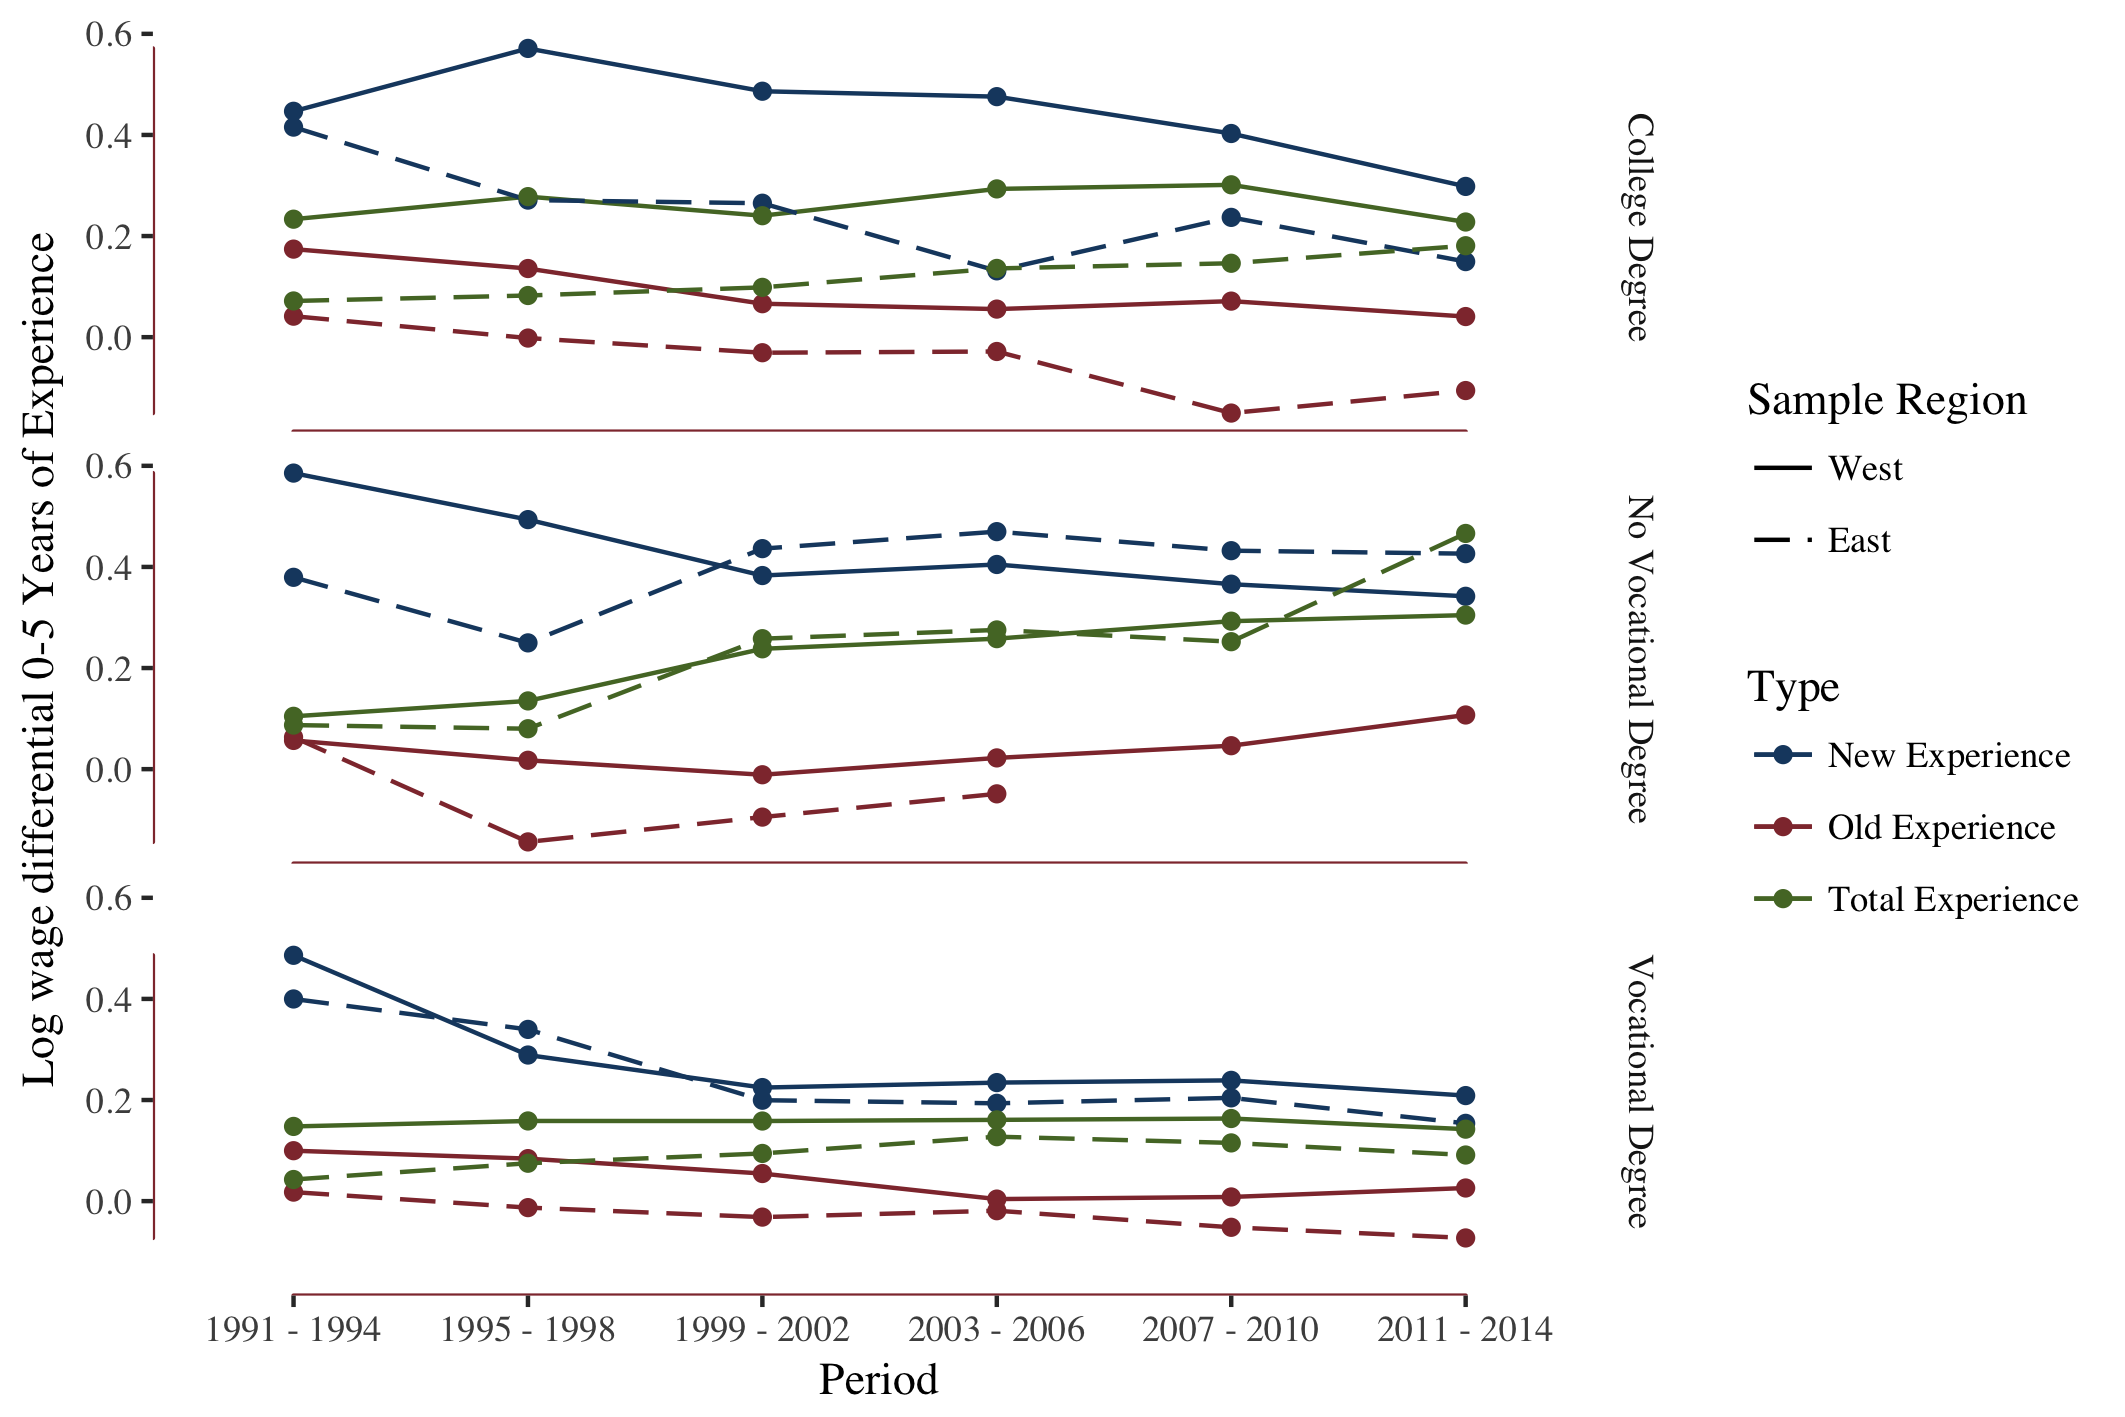
\includegraphics[width=\textwidth]{/Users/Christian/Statistik_Studium/EconProject/Code/Graphics/plotDiffComparisonExpBySkillGroup.png}
    \caption{Predicted Log Wage Difference 5-0 Years of Experience}
    \label{fig:DiffComparisonExpBySkillGroup}
\end{figure}

\begin{figure}[!h]
    \centering
    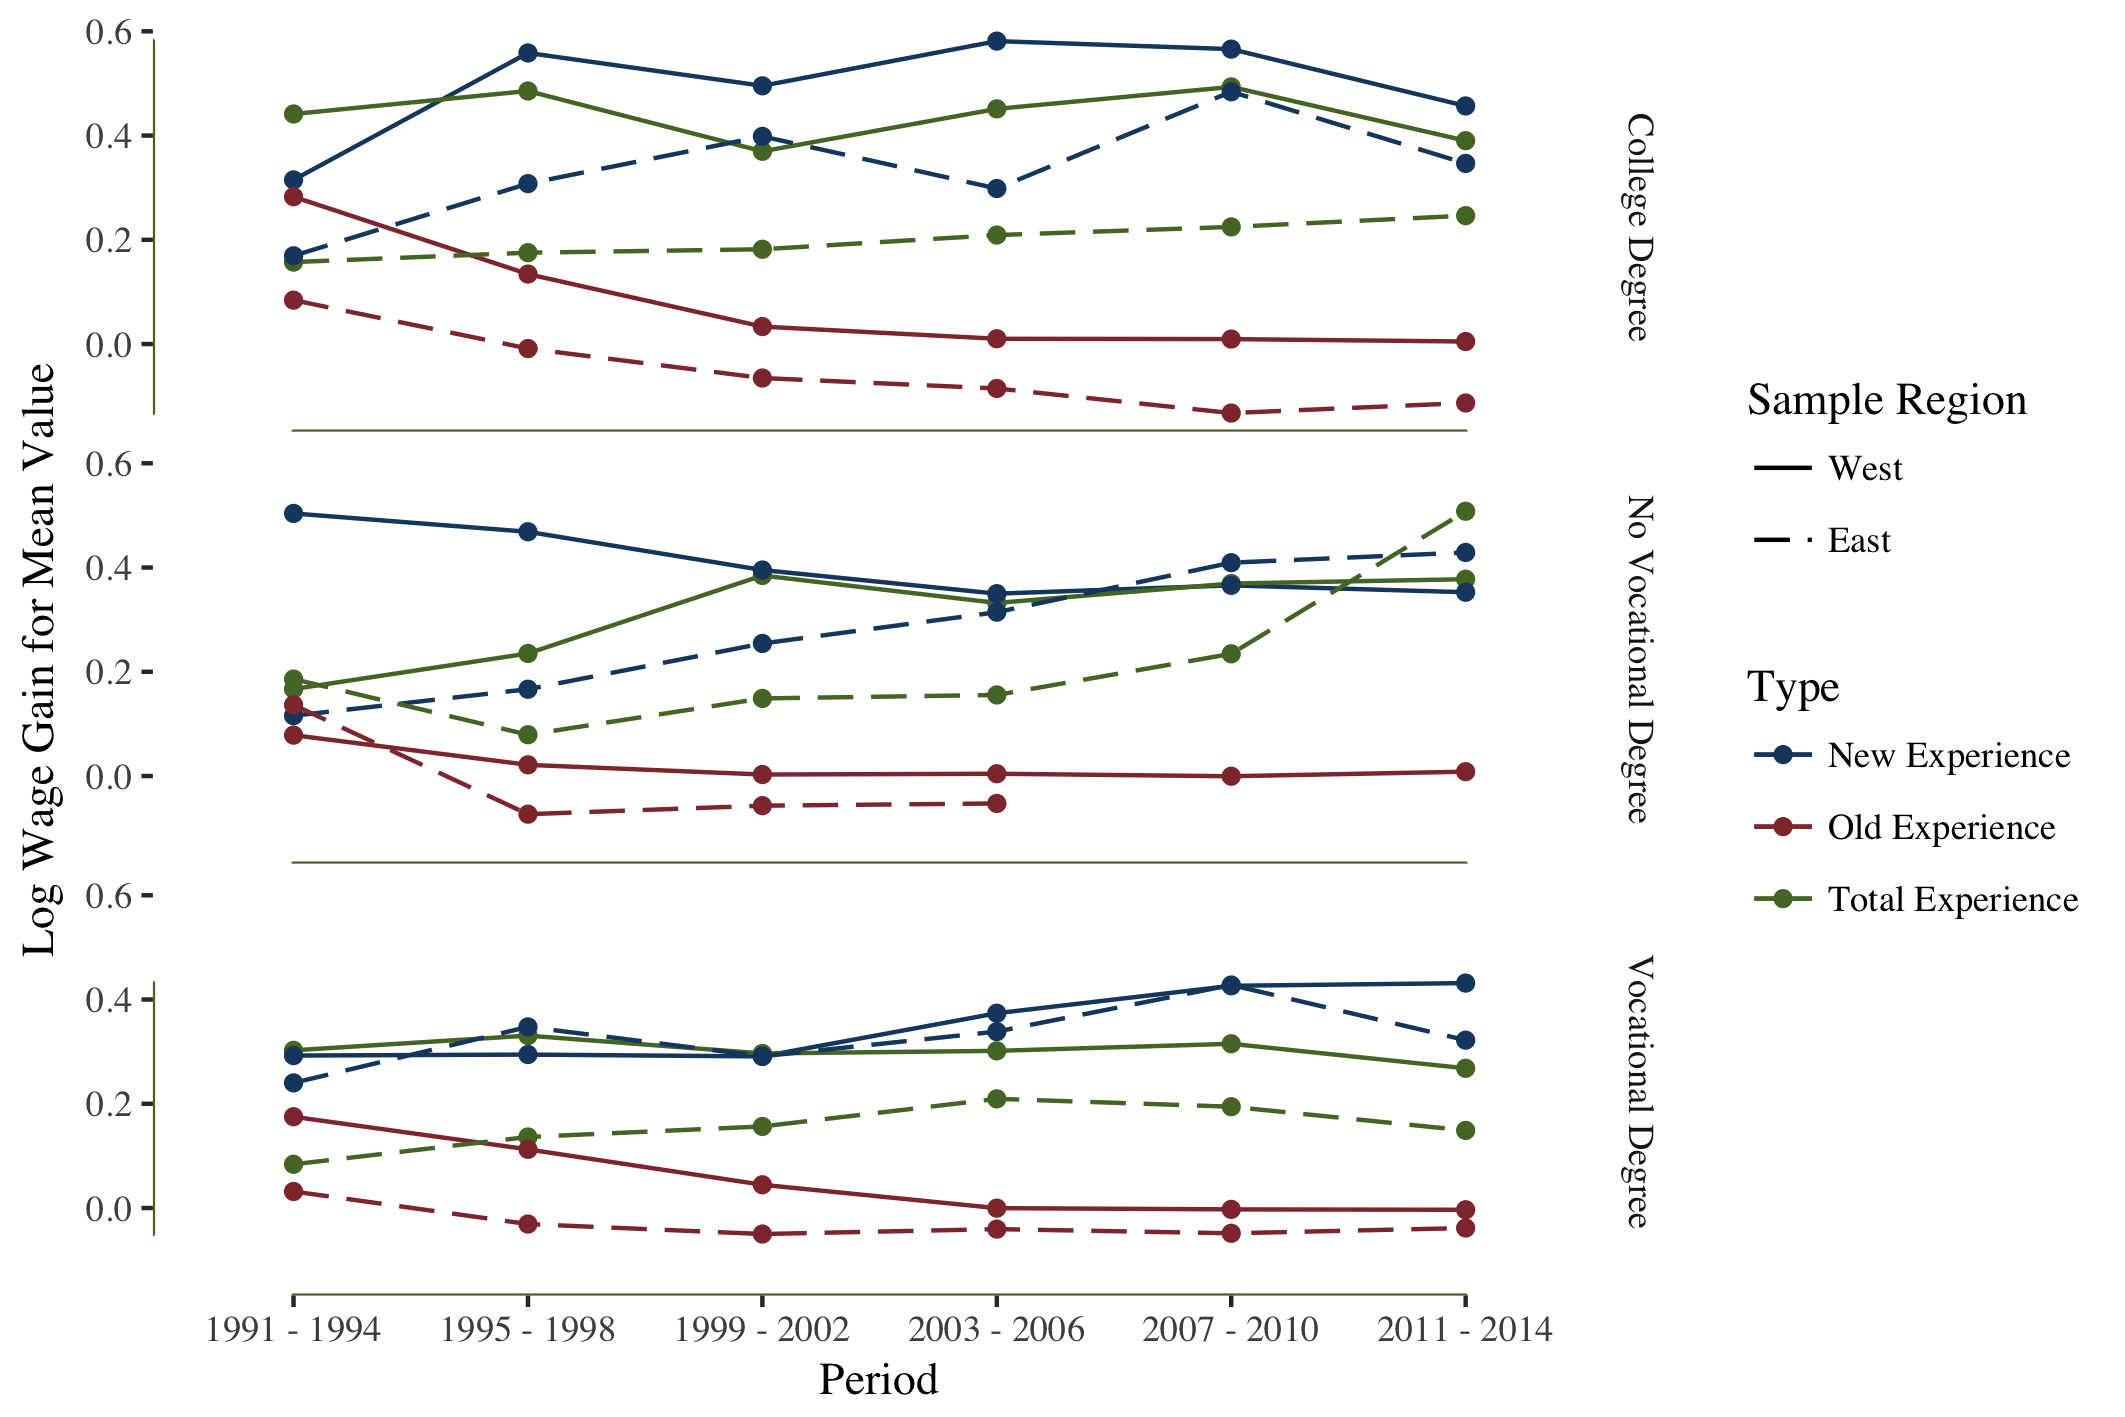
\includegraphics[width=\textwidth]{/Users/Christian/Statistik_Studium/EconProject/Code/Graphics/plotHumanCapitalExpBySkillGroup.png}
    \caption{Predicted Log Wage Difference for Mean Years of Experience separated by Skill Group}
    \label{fig:HumanCapitalExpBySkillGroup}
\end{figure}
\FloatBarrier

\section{Conclusions}
From the above evidence one might draw the following conclusions:
\begin{enumerate}
	\item Old Experience gathered in East Germany is practically without value on the post unification labour market, whereas those gathered in West Germany retained some value up until the late nineties.
	\item Returns to Education are similar across type (Old/New) and Region. Also they are rising throughout the time frame.
	\item East German individuals seem to have higher share of their Human Capital stored in Education, specifically Old Education. This seems at least partly driven by higher education levels in the East German sample and a higher proportion of Old Education.
	\item Returns to New Experience are consistently higher in West Germany. 
	\item The decreasing difference in returns to Total Experience (and responding Human Capital) in the nineties seems mainly due to the vanishing influence of different valuations of Old Experience. The remaining gap however seems mainly due to the difference in evaluation of New Experience and does not show a clear trend of disappearing.
	\item In the nineties Returns to New Experience differed significantly for both College Graduates and individuals wit No Vocational Degree. Whereas this difference has vanished for the latter git has decreased much slower for the former and remains significant. Differences in the returns to experience for individuals with vocational degree are relatively small throughout the time frame.
	\item The difference in human capital from New Experience seems to be concentrated in the group of people with College Degree.
\end{enumerate}

\section{Coefficients}

\begin{table}
\begin{center}
\begin{small}
\begin{tabular}{l c c c c c c }
\hline
 & 1991 - 1994 & 1995 - 1998 & 1999 - 2002 & 2003 - 2006 & 2007 - 2010 & 2011 - 2014 \\
\hline
(Intercept)     & $6.8089^{***}$  & $6.8152^{***}$  & $6.6882^{***}$  & $6.6057^{***}$  & $6.4610^{***}$  & $6.4816^{***}$  \\
                & $(0.0199)$      & $(0.0223)$      & $(0.0239)$      & $(0.0257)$      & $(0.0258)$      & $(0.0249)$      \\
TotalEdu        & $0.0714^{***}$  & $0.0672^{***}$  & $0.0754^{***}$  & $0.0791^{***}$  & $0.0836^{***}$  & $0.0845^{***}$  \\
                & $(0.0014)$      & $(0.0014)$      & $(0.0015)$      & $(0.0016)$      & $(0.0016)$      & $(0.0016)$      \\
TotalExp        & $0.0332^{***}$  & $0.0388^{***}$  & $0.0408^{***}$  & $0.0459^{***}$  & $0.0466^{***}$  & $0.0409^{***}$  \\
                & $(0.0011)$      & $(0.0012)$      & $(0.0013)$      & $(0.0015)$      & $(0.0015)$      & $(0.0014)$      \\
TotalExpSquared & $-0.0006^{***}$ & $-0.0008^{***}$ & $-0.0008^{***}$ & $-0.0009^{***}$ & $-0.0009^{***}$ & $-0.0008^{***}$ \\
                & $(0.0000)$      & $(0.0000)$      & $(0.0000)$      & $(0.0000)$      & $(0.0000)$      & $(0.0000)$      \\
Tenure          & $0.0022^{***}$  & $0.0026^{***}$  & $0.0029^{***}$  & $0.0045^{***}$  & $0.0053^{***}$  & $0.0053^{***}$  \\
                & $(0.0005)$      & $(0.0005)$      & $(0.0006)$      & $(0.0007)$      & $(0.0007)$      & $(0.0007)$      \\
sex[2] weiblich & $-0.2701^{***}$ & $-0.2367^{***}$ & $-0.2321^{***}$ & $-0.2001^{***}$ & $-0.1846^{***}$ & $-0.2040^{***}$ \\
                & $(0.0078)$      & $(0.0085)$      & $(0.0090)$      & $(0.0096)$      & $(0.0099)$      & $(0.0095)$      \\
\hline
R$^2$           & 0.3823          & 0.3623          & 0.3821          & 0.3727          & 0.3974          & 0.3898          \\
Adj. R$^2$      & 0.3818          & 0.3618          & 0.3815          & 0.3721          & 0.3968          & 0.3892          \\
Num. obs.       & 10383           & 9016            & 8769            & 8483            & 7947            & 8488            \\
RMSE            & 0.3463          & 0.3530          & 0.3848          & 0.4107          & 0.4070          & 0.4096          \\
\hline
\multicolumn{7}{l}{\tiny{$^{***}p<0.001$, $^{**}p<0.01$, $^*p<0.05$}}
\end{tabular}
\end{small}
\caption{Model Coefficients for West German Data using Model 1}
\label{table:WestModelsTotal}
\end{center}
\end{table}


\begin{table}
\begin{center}
\begin{small}
\begin{tabular}{l c c c c c c }
\hline
 & 1991 - 1994 & 1995 - 1998 & 1999 - 2002 & 2003 - 2006 & 2007 - 2010 & 2011 - 2014 \\
\hline
(Intercept)     & $6.2025^{***}$  & $6.5169^{***}$  & $6.4577^{***}$  & $6.2844^{***}$  & $6.1174^{***}$  & $6.1040^{***}$  \\
                & $(0.0255)$      & $(0.0292)$      & $(0.0312)$      & $(0.0378)$      & $(0.0432)$      & $(0.0404)$      \\
TotalEdu        & $0.0640^{***}$  & $0.0676^{***}$  & $0.0737^{***}$  & $0.0862^{***}$  & $0.0929^{***}$  & $0.0957^{***}$  \\
                & $(0.0017)$      & $(0.0020)$      & $(0.0022)$      & $(0.0026)$      & $(0.0028)$      & $(0.0027)$      \\
TotalExp        & $0.0121^{***}$  & $0.0189^{***}$  & $0.0242^{***}$  & $0.0317^{***}$  & $0.0291^{***}$  & $0.0278^{***}$  \\
                & $(0.0014)$      & $(0.0016)$      & $(0.0016)$      & $(0.0020)$      & $(0.0024)$      & $(0.0022)$      \\
TotalExpSquared & $-0.0002^{***}$ & $-0.0004^{***}$ & $-0.0006^{***}$ & $-0.0007^{***}$ & $-0.0007^{***}$ & $-0.0007^{***}$ \\
                & $(0.0000)$      & $(0.0000)$      & $(0.0000)$      & $(0.0001)$      & $(0.0001)$      & $(0.0001)$      \\
Tenure          & $0.0017^{***}$  & $0.0075^{***}$  & $0.0084^{***}$  & $0.0094^{***}$  & $0.0114^{***}$  & $0.0132^{***}$  \\
                & $(0.0005)$      & $(0.0006)$      & $(0.0007)$      & $(0.0009)$      & $(0.0010)$      & $(0.0010)$      \\
sex[2] weiblich & $-0.1806^{***}$ & $-0.1304^{***}$ & $-0.1396^{***}$ & $-0.1747^{***}$ & $-0.1848^{***}$ & $-0.1661^{***}$ \\
                & $(0.0082)$      & $(0.0095)$      & $(0.0105)$      & $(0.0128)$      & $(0.0148)$      & $(0.0143)$      \\
\hline
R$^2$           & 0.3517          & 0.2423          & 0.2762          & 0.3056          & 0.2944          & 0.3474          \\
Adj. R$^2$      & 0.3510          & 0.2412          & 0.2750          & 0.3043          & 0.2930          & 0.3460          \\
Num. obs.       & 7242            & 5924            & 5155            & 4318            & 3927            & 3659            \\
RMSE            & 0.3430          & 0.3566          & 0.3688          & 0.4102          & 0.4459          & 0.4110          \\
\hline
\multicolumn{7}{l}{\tiny{$^{***}p<0.001$, $^{**}p<0.01$, $^*p<0.05$}}
\end{tabular}
\end{small}
\caption{Model Coefficients for East German Data using Model 1}
\label{table:EastModelsTotal}
\end{center}
\end{table}


\begin{table}
\begin{center}
\begin{small}
\begin{tabular}{l c c c c c c }
\hline
 & 1991 - 1994 & 1995 - 1998 & 1999 - 2002 & 2003 - 2006 & 2007 - 2010 & 2011 - 2014 \\
\hline
(Intercept)     & $6.7103^{***}$  & $6.6758^{***}$  & $6.6270^{***}$  & $6.5452^{***}$  & $6.4074^{***}$  & $6.3922^{***}$  \\
                & $(0.0241)$      & $(0.0296)$      & $(0.0282)$      & $(0.0314)$      & $(0.0319)$      & $(0.0295)$      \\
OldEdu          & $0.0727^{***}$  & $0.0691^{***}$  & $0.0756^{***}$  & $0.0781^{***}$  & $0.0816^{***}$  & $0.0809^{***}$  \\
                & $(0.0014)$      & $(0.0015)$      & $(0.0015)$      & $(0.0016)$      & $(0.0017)$      & $(0.0017)$      \\
NewEdu          & $0.0506^{***}$  & $0.0545^{***}$  & $0.0642^{***}$  & $0.0727^{***}$  & $0.0816^{***}$  & $0.0885^{***}$  \\
                & $(0.0067)$      & $(0.0039)$      & $(0.0026)$      & $(0.0024)$      & $(0.0022)$      & $(0.0019)$      \\
OldExp          & $0.0222^{***}$  & $0.0175^{***}$  & $0.0109^{***}$  & $0.0037$        & $0.0058^{*}$    & $0.0105^{**}$   \\
                & $(0.0011)$      & $(0.0013)$      & $(0.0017)$      & $(0.0023)$      & $(0.0027)$      & $(0.0034)$      \\
OldExpSquared   & $-0.0005^{***}$ & $-0.0004^{***}$ & $-0.0003^{***}$ & $-0.0002^{*}$   & $-0.0004^{**}$  & $-0.0008^{***}$ \\
                & $(0.0000)$      & $(0.0000)$      & $(0.0001)$      & $(0.0001)$      & $(0.0001)$      & $(0.0002)$      \\
NewExp          & $0.2374^{***}$  & $0.1156^{***}$  & $0.0839^{***}$  & $0.0803^{***}$  & $0.0690^{***}$  & $0.0561^{***}$  \\
                & $(0.0207)$      & $(0.0096)$      & $(0.0056)$      & $(0.0047)$      & $(0.0038)$      & $(0.0029)$      \\
NewExpSquared   & $-0.0272^{***}$ & $-0.0066^{***}$ & $-0.0036^{***}$ & $-0.0026^{***}$ & $-0.0019^{***}$ & $-0.0012^{***}$ \\
                & $(0.0044)$      & $(0.0011)$      & $(0.0004)$      & $(0.0003)$      & $(0.0002)$      & $(0.0001)$      \\
Tenure          & $0.0020^{***}$  & $0.0021^{***}$  & $0.0026^{***}$  & $0.0045^{***}$  & $0.0052^{***}$  & $0.0054^{***}$  \\
                & $(0.0005)$      & $(0.0005)$      & $(0.0006)$      & $(0.0007)$      & $(0.0007)$      & $(0.0007)$      \\
sex[2] weiblich & $-0.2651^{***}$ & $-0.2240^{***}$ & $-0.2155^{***}$ & $-0.1804^{***}$ & $-0.1686^{***}$ & $-0.1920^{***}$ \\
                & $(0.0077)$      & $(0.0085)$      & $(0.0090)$      & $(0.0096)$      & $(0.0100)$      & $(0.0096)$      \\
\hline
R$^2$           & 0.4005          & 0.3791          & 0.4000          & 0.3913          & 0.4082          & 0.3980          \\
Adj. R$^2$      & 0.3999          & 0.3784          & 0.3993          & 0.3905          & 0.4074          & 0.3973          \\
Num. obs.       & 10383           & 9016            & 8769            & 8483            & 7947            & 8488            \\
RMSE            & 0.3413          & 0.3483          & 0.3793          & 0.4046          & 0.4034          & 0.4069          \\
\hline
\multicolumn{7}{l}{\tiny{$^{***}p<0.001$, $^{**}p<0.01$, $^*p<0.05$}}
\end{tabular}
\end{small}
\caption{Model Coefficients for West German Data using Model 2}
\label{table:WestModelsOldNew}
\end{center}
\end{table}


\begin{table}
\begin{center}
\begin{small}
\begin{tabular}{l c c c c c c }
\hline
 & 1991 - 1994 & 1995 - 1998 & 1999 - 2002 & 2003 - 2006 & 2007 - 2010 & 2011 - 2014 \\
\hline
(Intercept)     & $6.1512^{***}$  & $6.4542^{***}$  & $6.4373^{***}$  & $6.2883^{***}$  & $6.0307^{***}$  & $6.0872^{***}$  \\
                & $(0.0304)$      & $(0.0384)$      & $(0.0391)$      & $(0.0490)$      & $(0.0552)$      & $(0.0492)$      \\
OldEdu          & $0.0639^{***}$  & $0.0674^{***}$  & $0.0734^{***}$  & $0.0855^{***}$  & $0.0899^{***}$  & $0.0933^{***}$  \\
                & $(0.0017)$      & $(0.0020)$      & $(0.0022)$      & $(0.0026)$      & $(0.0029)$      & $(0.0028)$      \\
NewEdu          & $0.0219$        & $0.0453^{***}$  & $0.0622^{***}$  & $0.0828^{***}$  & $0.0977^{***}$  & $0.0960^{***}$  \\
                & $(0.0121)$      & $(0.0064)$      & $(0.0041)$      & $(0.0039)$      & $(0.0037)$      & $(0.0032)$      \\
OldExp          & $0.0058^{***}$  & $-0.0035^{*}$   & $-0.0066^{**}$  & $-0.0014$       & $-0.0188^{***}$ & $-0.0191^{***}$ \\
                & $(0.0014)$      & $(0.0017)$      & $(0.0022)$      & $(0.0031)$      & $(0.0042)$      & $(0.0049)$      \\
OldExpSquared   & $-0.0001^{**}$  & $0.0001$        & $0.0000$        & $-0.0003^{**}$  & $0.0003$        & $0.0001$        \\
                & $(0.0000)$      & $(0.0001)$      & $(0.0001)$      & $(0.0001)$      & $(0.0002)$      & $(0.0003)$      \\
NewExp          & $0.1555^{***}$  & $0.0706^{***}$  & $0.0510^{***}$  & $0.0403^{***}$  & $0.0445^{***}$  & $0.0324^{***}$  \\
                & $(0.0284)$      & $(0.0131)$      & $(0.0082)$      & $(0.0075)$      & $(0.0066)$      & $(0.0049)$      \\
NewExpSquared   & $-0.0138^{*}$   & $-0.0009$       & $-0.0011$       & $-0.0006$       & $-0.0005$       & $-0.0005^{**}$  \\
                & $(0.0063)$      & $(0.0015)$      & $(0.0006)$      & $(0.0004)$      & $(0.0003)$      & $(0.0002)$      \\
Tenure          & $0.0010^{*}$    & $0.0053^{***}$  & $0.0061^{***}$  & $0.0072^{***}$  & $0.0079^{***}$  & $0.0108^{***}$  \\
                & $(0.0005)$      & $(0.0006)$      & $(0.0007)$      & $(0.0009)$      & $(0.0011)$      & $(0.0010)$      \\
sex[2] weiblich & $-0.1673^{***}$ & $-0.1027^{***}$ & $-0.1133^{***}$ & $-0.1504^{***}$ & $-0.1484^{***}$ & $-0.1424^{***}$ \\
                & $(0.0083)$      & $(0.0094)$      & $(0.0105)$      & $(0.0129)$      & $(0.0149)$      & $(0.0144)$      \\
\hline
R$^2$           & 0.3637          & 0.2808          & 0.3054          & 0.3228          & 0.3195          & 0.3630          \\
Adj. R$^2$      & 0.3628          & 0.2794          & 0.3039          & 0.3210          & 0.3176          & 0.3611          \\
Num. obs.       & 7242            & 5924            & 5155            & 4318            & 3927            & 3659            \\
RMSE            & 0.3399          & 0.3475          & 0.3614          & 0.4052          & 0.4381          & 0.4062          \\
\hline
\multicolumn{7}{l}{\tiny{$^{***}p<0.001$, $^{**}p<0.01$, $^*p<0.05$}}
\end{tabular}
\end{small}
\caption{Model Coefficients for East German Data using Model 2}
\label{table:EastModelsOldNew}
\end{center}
\end{table}

\bibliography{EconometricProject}

\end{document}


